\documentclass[
%draft%     uncomment to activate draft mode (see preamble/proofs)
]{scrbook}   

% preamble -- do not rearrange order of \includes
\KOMAoptions{
    titlepage=false,
    paper=150mm:220mm,
    twoside=true, 
    twocolumn=false,
    toc=chapterentryfill,       % for dots: chapterentrydotfill
    parskip=false,              % space between paragraphs. "full" gives more space; "false" uses indentation instead
    headings=small,
    draft=false,                % switch to "true" to activate draftmode
    bibliography=leveldown,     % turns the Bibliography into a \section rather than a \chapter (so it appears on the same page)
}

\usepackage[
    top=23mm,
    left=20mm,
    height=173mm,
    width=109mm,
    ]{geometry}

\setlength{\marginparwidth}{2cm} % sets up acceptable margin for \todonotes package (see preamble/packages.tex).
\usepackage[dvipsnames]{xcolor}
\usepackage[unicode]{hyperref}  % hyperlinks
\usepackage{booktabs}           % professional-quality tables
\usepackage{nicefrac}           % compact symbols for 1/2, etc.
\usepackage{microtype}          % microtypography
\usepackage{lipsum}             % lorem ipsum at the ready
\usepackage{graphicx}           % for figures
\usepackage{footmisc}           % makes symbol footnotes possible
\usepackage{ragged2e}
\usepackage{changepage}         % detect odd/even pages
\usepackage{array}
\usepackage{float}              % get figures etc. to stay where they are with [H]
\usepackage{subfigure}          % \subfigures witin a \begin{figure}
\usepackage{longtable}          % allows for tables that stretch over multiple pages
\setlength{\marginparwidth}{2cm}
\usepackage[textsize=footnotesize]{todonotes} % enables \todo's for editors
\usepackage{etoolbox}           % supplies commands like \AtBeginEnvironment and \atEndEnvironment
\usepackage{ifdraft}            % switches on proofreading options in the draft mode
\usepackage{rotating}           % provides sidewaysfigure environment
\usepackage{media9}             % allows for video in the pdf
\usepackage{xurl}               % allows URLs to (line)break ANYWHERE


\usepackage[L7x, T1]{fontenc}           % use 8-bit T1 fonts
\usepackage[utf8]{inputenc}             % allow utf-8 input
% languages
\usepackage[main=english, lithuanian, latin]{babel}
% special characters
\DeclareUnicodeCharacter{2D7}{}         % allow ¡ character
\DeclareUnicodeCharacter{45E}{}         % allow ў character
\DeclareUnicodeCharacter{2032}{}        % allow ′ character
\DeclareUnicodeCharacter{22EE}{}        % allow ⋮ character
\usepackage{textalpha}                  % allows for greek characters in text e.g. \textalpha = α
\usepackage{textcomp}                   % allows \textrightarrow etc.

         
% Palatino font options
\usepackage{mathpazo}                   % Palatino in LaTeX math
\usepackage{tgpagella}                  % Palatino font
\addtokomafont{disposition}{\rmfamily}  % Palatino for titles etc.
\setkomafont{descriptionlabel}{         % font for description lists    
\usekomafont{captionlabel}\bfseries     % Palatino bold
}
\setkomafont{caption}{\footnotesize}    % smaller font size for captions

% To make sure LaTeX keeps using Palatino in Lithuanian:
% in OVERLEAF change the following \newcommand to \renewcommand
% \newcommand{\ltfamily}{\familydefault} 

% No (sub)sections in TOC
\setcounter{tocdepth}{0}                

% Redefines chapter title formatting
\makeatletter                               
\def\@makechapterhead#1{
  \vspace*{50\p@}%
  {\parindent \z@ \normalfont
    \interlinepenalty\@M
    \Large\raggedright #1\par\nobreak%
    \vskip 40\p@%
  }}
\makeatother
% a bit more space between titles and page numbers in TOC

\makeatletter   
\renewcommand\@pnumwidth{2.5em} 
\makeatother

% Title and Author of individual contributions
\makeatletter
% paper/review author = contributor
\newcommand\contributor[1]{\renewcommand\@contributor{#1}}
\newcommand\@contributor{}
\newcommand\thecontributor{\@contributor} 
% paper/review title = contribution
\newcommand\contribution[1]{\renewcommand\@contribution{#1}}
\newcommand\@contribution{}
\newcommand\thecontribution{\@contribution}
% short contributor for running header
\newcommand\shortcontributor[1]{\renewcommand\@shortcontributor{#1}}
\newcommand\@shortcontributor{}
\newcommand\theshortcontributor{\@shortcontributor} 
% short title for running header
\newcommand\shortcontribution[1]{\renewcommand\@shortcontribution{#1}}
\newcommand\@shortcontribution{}
\newcommand\theshortcontribution{\@shortcontribution}
\makeatother
% choose copyright license
\usepackage[               
    type={CC},
    modifier={by},
    version={4.0},
]{doclicense}

% define \copyrightstatement for ease of use
\newcommand{\copyrightstatement}{
         \doclicenseIcon \ \theyear. 
         \doclicenseLongText            % includes a link
}

\usepackage[sort&compress,semicolon,authoryear,elide]{natbib} % for citations
\usepackage{chapterbib}
\bibliographystyle{variants}
\setcitestyle{notesep={, },aysep={}, yysep={;}}
% Environments
\AtBeginEnvironment{quote}{\footnotesize\vskip 1em}
\AtEndEnvironment{quote}{\vskip 1em}

\setkomafont{caption}{\footnotesize}

% Preface
\newenvironment{preface}{
    \phantomsection
    \cleardoublepage
    \addcontentsline{toc}{part}{Editors' Preface}
    % enable running title
    \pagestyle{preface}
    % \chapter*{Editors' Preface}    
    % reset the section counter for each paper
    \setcounter{section}{0}  
    % no running title on first page, page number center bottom instead
    \thispagestyle{chaptertitlepage}
}{}
\AtEndEnvironment{preface}{%
    %last page running header fix
    \protect\thispagestyle{preface}
}
% Essays
\newenvironment{paper}{
    \phantomsection
    % start every new paper on an uneven page 
    \cleardoublepage
    % enable running title
    \pagestyle{fancy}
    % change section numbering FROM [\chapter].[\section].[\subsection] TO [\section].[\subsection] ETC.
    \renewcommand{\thesection}{\arabic{section}}
    % mark chapter % add author + title to the TOC
    \chapter[\normalfont\textbf{\emph{\thecontributor}}: \thecontribution]{\vspace{-4em}\Large\normalfont\thecontribution\linebreak\normalsize\begin{flushright}\emph{\thecontributor}\end{flushright}}    
    % reset the section counter for each paper
    \setcounter{section}{0}  
    % no running title on first page, page number center bottom instead, include copyright statement
    \thispagestyle{contributiontitlepage}
    % formatting for the bibliography
    \bibliographystyle{humannat}

}{}
\AtBeginEnvironment{paper}{
    % keeps running title from the first page:
    \renewcommand*{\pagemark}{}%                            
}
\AtEndEnvironment{paper}{
    % last page running header fix
    \protect\thispagestyle{fancy}%                              
}
% Reviews
\newenvironment{review}{
    \phantomsection
    % start every new paper on an uneven page 
    \cleardoublepage
    % enable running title
    \pagestyle{reviews}
    % change section numbering FROM [\chapter].[\section].[\subsection] TO [\section].[\subsection] ETC.
    \renewcommand{\thesection}{\arabic{section}} 
    % mark chapter % add author + title to the TOC
    \chapter[\normalfont\textbf{\emph{\thecontributor}}: \thecontribution]{}    % reset the section counter for each paper
    \setcounter{section}{0}  
    % no running title on first page, page number center bottom instead, include copyright statement
    \thispagestyle{contributiontitlepage}
    % formatting for the bibliography
    \bibliographystyle{humannat}
}{}
\AtBeginEnvironment{review}{
% keeps running title from the first page
    \renewcommand*{\pagemark}{}%                                   
}
\AtEndEnvironment{review}{
    % author name(s)
    \begin{flushright}\emph{\thecontributor}\end{flushright}
    % last page running header fix
    \protect\thispagestyle{reviews}                           
}

% Abstract
\newenvironment{abstract}{% 
\setlength{\parindent}{0pt} \begin{adjustwidth}{2em}{2em}\footnotesize\emph{\abstractname}: }{%
\vskip 1em\end{adjustwidth}
}{}

% Keywords
\newenvironment{keywords}{
\setlength{\parindent}{0pt} \begin{adjustwidth}{2em}{2em}\footnotesize\emph{Keywords}: }{%
\vskip 1em\end{adjustwidth}
}{}

% Review Abstract
\newenvironment{reviewed}{% 
\setlength{\parindent}{0pt}
    \begin{adjustwidth}{2em}{2em}\footnotesize}{%
\vskip 1em\end{adjustwidth}
}{}

% Motto
\newenvironment{motto}{% 
\setlength{\parindent}{0pt} \small\raggedleft}{%
\vskip 2em
}{}
% command for centering section headings
\newcommand{\centerheading}[1]{   
    \hspace*{\fill}#1\hspace*{\fill}
}

% Remove "Part #." from \part titles
% KOMA default: \newcommand*{\partformat}{\partname~\thepart\autodot}
\renewcommand*{\partformat}{} 

% No dots after figure or table numbers
\renewcommand*{\figureformat}{\figurename~\thefigure}
\renewcommand*{\tableformat}{\tablename~\thetable}

% paragraph handling
\setparsizes%
    {1em}% indent
    {0pt}% maximum space between paragraphs
    {0pt plus 1fil}% last line not justified
    

% In the "Authors" section, author names are put in the \paragraph{} headings. To reduce the space after these  headings, the default {-1em} has been changed to {-.4em} below.
\makeatletter
\renewcommand\paragraph{\@startsection {paragraph}{4}{\z@ }{3.25ex \@plus 1ex \@minus .2ex}{-.4em}{\normalfont \normalsize \bfseries }
}
\makeatother

% add the following (uncommented) in environments where you want to count paragraph numbers in the margin
%    \renewcommand*{\paragraphformat}{%
%    \makebox[-4pt][r]{\footnotesize\theparagraph\autodot\enskip}
%    }
%    \renewcommand{\theparagraph}{\arabic{paragraph}}
%    \setcounter{paragraph}{0}
%    \setcounter{secnumdepth}{4}
    
% running title
\RequirePackage{fancyhdr}
% cuts off running titles that are too long
%\RequirePackage{truncate}
% makes header as wide as geometry (SET SAME AS \TEXTWIDTH!)
\setlength{\headwidth}{109mm} 
% LO = Left Odd
\fancyhead[LO]{\small\emph{\theshortcontributor} \hspace*{.5em} \theshortcontribution} 
% RE = Right Even
\fancyhead[RE]{\sc{\small\theissue}}
% LE = Left Even
\fancyhead[LE]{\small\thepage}            
% RE = Right Odd
\fancyhead[RO]{\small\thepage}    
\fancyfoot{}
% no line under running title; cannot be \@z but needs to be 0pt
\renewcommand{\headrulewidth}{0 pt} 

% special style for authors pages
\fancypagestyle{authors}{
    \fancyhead[LO]{\small\textit{Authors}} 
    \fancyhead[LE]{\small\thepage}            
    \fancyhead[RE]{\sc{\small\theissue}}
    \fancyhead[RO]{\small\thepage}            
    \fancyfoot{}
}

% special style for book reviews
\fancypagestyle{reviews}{
    \fancyhead[LO]{\small\textit{Book Reviews}} 
    \fancyhead[LE]{\small\thepage}            
    \fancyhead[RE]{\sc{\small\theissue}}
    \fancyhead[RO]{\small\thepage}            
    \fancyfoot{}
}

% special style for Editors' preface.
\fancypagestyle{preface}{
    \fancyhead[LO]{\small\textit{Editors' Preface}} 
    \fancyhead[LE]{\small\thepage}            
    \fancyhead[RE]{\sc{\small\theissue}}
    \fancyhead[RO]{\small\thepage}            
    \fancyfoot{}
}
% special style for first pages of contributions etc.
% DOES include copyright statement
\fancypagestyle{contributiontitlepage}{
    \fancyhead[C]{\scriptsize\centering\copyrightstatement}
    \fancyhead[L,R]{}
    \fancyfoot[CE,CO]{\small\thepage}
}
% special style for first pages of other \chapters.
% DOES NOT include copyright statement
\fancypagestyle{chaptertitlepage}{
    \fancyhead[C,L,R]{}
    \fancyfoot[CE,CO]{\small\thepage}
}
% no page numbers on \part pages 
\renewcommand*{\partpagestyle}{empty}
% footnotes
\renewcommand{\footnoterule}{%
    \kern .5em  % call this kerna
    \hrule height 0.4pt width .2\columnwidth    % the .2 value made the footnote ruler (horizontal line) smaller (was at .4)
    \kern .5em % call this kernb
}
\usepackage{footmisc}               
\renewcommand{\footnotelayout}{
    \hspace{1.5em}    % space between footnote mark and footnote text
}    
\newcommand{\mytodo}[1]{\textcolor{red}{#1}}
% colours for code notations
\usepackage{listings}       
	\renewcommand\lstlistingname{Quelltext} 
	\lstset{                    % basic formatting (bash etc.)
	       basicstyle=\ttfamily,
 	       showstringspaces=false,
	       commentstyle=\color{BrickRed},
	       keywordstyle=\color{RoyalBlue}
	}
	\lstdefinelanguage{XML}{     % specific XML formatting overrides
		  basicstyle=\ttfamily,
		  morestring=[s]{"}{"},
		  morecomment=[s]{?}{?},
		  morecomment=[s]{!--}{--},
		  commentstyle=\color{OliveGreen},
		  moredelim=[s][\color{Black}]{>}{<},
		  moredelim=[s][\color{RawSienna}]{\ }{=},
		  stringstyle=\color{RoyalBlue},
 		  identifierstyle=\color{Plum}
	}
    % HOW TO USE? BASH EXAMPLE
    %   \begin{lstlisting}[language=bash]
    %   #some comment
    %   cd Documents
    %   \end{lstlisting}
\usepackage{ifdraft}
% uncommenting line 2 in main.tex will activate the following proof formatting:

\ifdraft{
%
% 1. Add a watermark
%
    \usepackage{draftwatermark} 
    \SetWatermarkText{PROOFS}       
%
% 2. Add line numbers
%
% !! UNCOMMENT WITH CAUTION !! 
% The following option throws nasty errors in OVERLEAF, that are only solved after the servers reset (overnight). 
% It does seem to work in TeXShop. 
% 
%    \usepackage[switch, modulo, pagewise]{lineno} 
%    \linenumbers                   
}{}                                      

% this alternative doesn't work yet...
%\makeatletter
% \newsavebox{\@linebox}
% \savebox{\@linebox}[3em][t]{\parbox[t]{3em}{%
%   \@tempcnta\@ne\relax
%   \loop{\underline{\scriptsize\the\@tempcnta}}\\
%     \advance\@tempcnta by \@ne\ifnum\@tempcnta<48\repeat}}
%\makeatother     

% define issue details
\newcommand\thejournal{My Journal}
\newcommand\thejournalsubtitle{A LaTeX Template for a Journal in the Humanities}
\newcommand\thevolume{1}
\newcommand\theseason{Autumn}
\newcommand\theyear{2019}
\newcommand\theissue{\thejournal \ \thevolume \ (\theyear)} 
\newcommand\thewebsite{https://my.journal.org}

\begin{document}
\sloppy                         % preferences more space between words over overrunning margins
\lefthyphenmin=3                % suppresses hyphenation after only 1 or 2 characters
                                % NB: You will need to repeat \lefthyphenmin in the text if you use \selectlanguage
\begin{titlepage}
\pagenumbering{gobble}
\begin{center}
\LARGE \textbf{\thejournal} \\ \thevolume
\vskip 1em
\Large \theseason \ \theyear
\vskip 2em
\normalsize
\textbf{General Editor}\\
\generaleditor\par
\vskip 1em
\textbf{Associate Editor}\\
\associateeditor\par
\vskip 1em
\textbf{Editorial Board}\par
Anonymous Board Member 1 \\
Anonymous Board Member 2 \\

\end{center}
\end{titlepage}

\date{}
\begin{titlepage}
\begin{center}
\pagenumbering{gobble}
\LARGE \textsc{\thejournal:  \thejournalsubtitle}
\vfill 
\large \textsc{General Editor} \\ Jane Doe \vskip 1em 
\large \textsc{Associate Editor} \\ John Doe
\vfill
\end{center}
\end{titlepage}

\null\vfill\small
\noindent\thejournal \ \thevolume. \thejournalsubtitle. \\ \par
% \noindent ISSN \\ \par
\noindent\doclicenseIcon \ \theyear \\ \par 
\noindent This volume, including all its contents, is licensed under a \doclicenseLongNameRef \ license, and made available in Open Access at \href{\thewebsite}{\thewebsite}. The authors of the individual contributions, who are identified as such, retain the copyright over their original work.  \\ \par
\noindent For more information on the \doclicenseNameRef license, please refer to: \\ \doclicenseURL.  \\ \par

\noindent This volume was typeset in \LaTeX~by [TYPESETTER] using \href{https://github.com/WoutDLN/variantx}{VariantX} --- a reusable template for journals in the Humanities, developed by Wout Dillen. VariantX is open source, available on GitHub, and deposited in the \href{https://about.zenodo.org}{Zenodo Open Science Repository}. DOI: \href{https://zenodo.org/record/3484652#.X0PdDy2w3kI}{10.5281/zenodo.3484652}.  
\newpage
\pagenumbering{roman}           
\tableofcontents  
\thispagestyle{empty}

% \include{essays/preface}
\pagenumbering{arabic}
\part{Essays}
%%%%%%%%%%%%%%
%% METADATA %%
%%%%%%%%%%%%%%

\contributor{
% Add all authors
Firstname Lastname, Firstname Lastname, etc.
}

\contribution{
% Add full title
Essay Title. Subtitle.
}

\shortcontributor{
% short version of authors for running header
Lastname et al.
}

\shortcontribution{
% short version of title for running header
Short Title
}

\begin{paper}
\renewcommand*{\pagemark}{}

\begin{abstract}
% write your abstract here
Sample Abstract.
\end{abstract}

%%%%%%%%%%%%%%%%%%%%%%%%%%%%
%% YOUR ESSAY STARTS HERE %%
%%%%%%%%%%%%%%%%%%%%%%%%%%%%

% remove asterisk (*) if you want to number your sections
% add a title for your section in between the {curly brackets} if you need one
\section*{} 
Your Essay \citep{key}.

\end{paper}
\contributor{Merisa Martinez, Wout Dillen, Elli Bleeker, Anna-Maria Sichani, \mbox{and Aodhán Kelly}}
\contribution{Refining our Conceptions of
Access in Digital Scholarly Editing: Reflections on a Qualitative Survey
on Inclusive Design and Dissemination.}
\shortcontributor{Merisa Martinez et al.}
\shortcontribution{Refining our Conceptions of
Access}

\begin{paper}
\renewcommand{\thesubsection}{\arabic{subsection}}  

\begin{abstract}In this paper we explore layered conceptions of access and accessibility
as they relate to the theory and praxis of digital scholarly editing. To
do this, we designed and disseminated a qualitative survey on five key
themes: dissemination; Open Access and licensing; access to code; web
accessibility; and diversity. Throughout the article we engage in
cultural criticism of the discipline by sharing results from the survey,
identifying how the community talks about and performs access, and
pinpointing where improvements in praxis could be made. In the final
section of this paper we reflect on different ways to utilize the survey
results when critically designing and disseminating digital scholarly
editions, propose a call to action, and identify avenues of future
research.
\end{abstract}

%\begin{keywords}digital scholarly editing, access, accessibility, code, Open Access, dissemination, inclusive design, diversity, survey, cultural criticism, digital humanities \end{keywords}

\section*{Introduction\footnote{\textsc{Disclaimer.} This article was originally published in the \emph{Variants 14. The Journal of the European Society for Textual Scholarship}, and is purely published here, with the authors' consent, for demonstrative purposes. The process of transforming the article's references into BibTeX has introduced some minor variations in the text (layout and bibliography). If you would like to reference this article in your own research, please consult the original, which is available in Open Access here: \href{https://journals.openedition.org/variants/1070}{https://journals.openedition.org/variants/1070}.}}

\textsc{Access, in all its iterations}, continues to shape the discourse of
textual scholarship as the field grapples with new methods and models of
the digital scholarly edition (DSE).\footnote{The authors wish to
  acknowledge that the work for this article was funded in part by the
  Digital Scholarly Editions Innovative Training Network (DiXiT ITN), a
  Marie Sklodowska-Curie Action, underwritten by the EU Seventh
  Framework Programme (FP7/2007-2013), REA grant no. 317436.} Using an
amalgamation and paraphrasing of two definitions posed by Patrick
Sahle (\citeyear{sahle_catalog_2008,sahle_what_2016}), we define a digital scholarly edition as an
information resource which offers a critical representation of
(normally) historical documents or texts and which is guided by a
digital paradigm in its theory, method and practice. Discourse around
digital scholarly editions and conceptions of access has been ongoing
among textual scholars for the past twenty years. In \citeyear{lavagnino_access_2009}, John
Lavagnino reflected on editorial practice in 1997, citing the tension --
present even then --- between creating digital editions for a scholarly
audience and a broader readership. He notes that at the time, there were
few digital editions with elements that acted as ``an invitation to look
at the texts along with the editor'' \citep[67]{lavagnino_access_2009}. Summarizing
an argument made by Jerome McGann in 2001, Susan Schreibman writes that
``it was only when textual scholars had the opportunity of editing in a
medium other than the book that they were able to realize the
constraints of the medium imposed on them'' (\citeyear{schreibman_digital_2019}). The perceived
openness of the web, however, also brought a new set of challenges for
editors. The understanding of who exactly is involved in the creation of
editions expanded to include not just editors and publishers, but
students, software and web developers, computer scientists, librarians,
archivists, project managers, and digitization specialists. Indeed, as
Martha Nell Smith (\citeyear{smith_electronic_2004}) asserts, ``we have entered a different
editorial time, one that demands the conscious cultivation of many
hands, eyes, ears, and voices''. Perhaps the most notable change from
the analog to the digital has been the extended focus on users. Nell
Smith goes on to state that ``{[}w{]}hen editors make as much about a
text visible to as wide an audience as possible, rather than silencing
opposing views or establishing one definitive text over all others,
intellectual connections are more likely to be found than lost''. Such
discussions illustrate the history of accessibility issues for editors
who have moved from the well-established norms of the print paradigm to
the ever-changing digital publishing environment.

While ``accessibility'' is a highly-cited term in digital scholarly
editing, it generally refers to making data \citep{sahle_criteria_2014} or source
materials \citep[222]{martens_what_1995} available to users rather than to making
data more accessible to different types of users --- which is the
predominant definition of the term in the context of software and web
development \citep{w3c_accessibility_2018}. This basic distinction indicates that access is
a multilayered concept in the digital humanities and that to avoid
discussing the topic at cross-purposes further refinement of the term is
needed. This paper frames a discussion around a broader definition of
access in relation to digital textual scholarship by examining pertinent
questions in the field: What type(s) of materials do we make accessible
in our digital scholarly editions? How? And to whom? Answering these
questions will help us to pinpoint digital scholarly editing praxis as
it stands at the present time and to aid in the continued development of
praxis for a new generation of textual scholars who will work primarily,
if not solely, on \emph{digital} scholarly editions.

We address these issues by building on our panel
discussion at the Digital Humanities 2017 conference in Montréal, Canada
\citep{sichani_refining_2017}. At this event, we explored the concept of access
in the field of digital scholarly editing in terms of (web)
accessibility, usability, pedagogy, collaboration, community and
diversity. To gain some preliminary insights about community
perspectives before our panel, we released a qualitative survey on
inclusive \mbox{design} and dissemination in early July 2017. In return, we
received rich, nuanced data from the community and decided to leave the
survey open until November to attract more responses. Collecting and
interpreting this data allowed us to engage in much needed cultural
criticism of the discipline \citep{fiormonte_towards_2012,liu_where_2012,posner_whats_2016}
by encouraging practitioners within the digital scholarly editing
community to critically reflect on what the term ``access'' means in
both the literal and more abstract senses of the word.

During the process of aggregating and analysing survey responses from
the community, it was apparent that our dataset contained an interesting
array of approaches to access taken by a broad cross-section of
practitioners with different backgrounds in the field (albeit a sample
with a clear bias towards European and Northern American experiences, see Figure \ref{demographic}).
We aim to communicate a broad overview of these data and consider their
implications for the five thematic layers of access that were covered in
the survey: (1) dissemination, (2) Open Access and licensing issues, (3)
access to the code of the edition, (4) web accessibility and usability,
and (5) inclusivity and diversity.

\section*{Inclusive design and dissemination in Digital Scholarly
Editions: A survey}

Our survey, ``Inclusive Design and Dissemination in Digital Scholarly
Editions'', was designed and hosted using SurveyMonkey.\footnote{We have
  deposited a CSV file of the survey's raw data (uncorrected, but
  scrubbed of respondents' personal information, following GDPR
  compliance requirements) in the Open Access Humanities Commons
  repository, alongside an accompanying PDF file with graphical
  representations of the survey's statistics. The redacted datasets can
  be found here: \href{http://dx.doi.org/10.17613/c3m9-kq76}{http://dx.doi.org/10.17613/c3m9-kq76} (csv) and here: \href{http://dx.doi.org/10.17613/x4mx-x394}{http://dx.doi.org/10.17613/x4mx-x394} (pdf).}
The survey was conducted between July and November 2017. We distributed
it through a series of relevant mailing lists, social media portals, and
via personal emails to practitioners in the field in our own
networks.\footnote{The following mailing lists were used: Humanist
  Discussion Group; Digital \mbox{Library} Forum/Council on Library and
  Information Resources (DLF/CLIR); Text Encoding Initiative (TEI-L);
  CODE4LIB; Scholarly Editing Forum (SEDIT-L); Textual Scholarship;
  Association for Digital Humanities Organizations (ADHO); Society for
  the History of \mbox{Authorship}, Reading and Publishing (SHARP-L); Swedish
  School of Library and Information Science (SSLIS); Digital Humanities
  Benelux; Digital Humanities in Flanders (DHu.F); Digital Research
  Infrastructure in the Arts and Humanities-Belgium (DARIAH-BE); Nordic
  Network of Editions (NNE); Digital Humanities Summer Institute (DHSI);
  Global Outlook: Digital Humanities (GO:DH); the National Endowment for
  the Humanities (NEH)'s ``Make Your Edition'' workshop mailing list;
  and the Digital Scholarly Editing Innovative Training Network (DiXiT
  ITN).} In total we received 219 responses, 109 of which completed
every required question in the survey --- resulting in a completion rate
of 49.7\%. Given the length of the survey (with 42 questions distributed
over 14 pages, which most respondents took over 40 minutes to complete),
this was a healthy completion rate.\footnote{The duration was arrived at
  by comparing SurveyMonkey's ``Time Spent'' values for all respondents,
  which we rounded off to the closest half minute mark. This time does
  not necessarily reflect ``active'' time spent on completing survey
  answers, but measures the distance between the moment when respondents
  start and complete the survey. Values for completed surveys ranged
  between six minutes and over a week, and had median of 41.25 minutes.}
Taking into account that 65 of these 109 respondents (or almost 60\%)
expressed their willingness to participate in a follow-up interview, it
is clear that the issues raised in the survey are of considerable
interest to the community --- or, at least, to that portion of the
community that we were able to reach with our survey.

\begin{figure}[H]
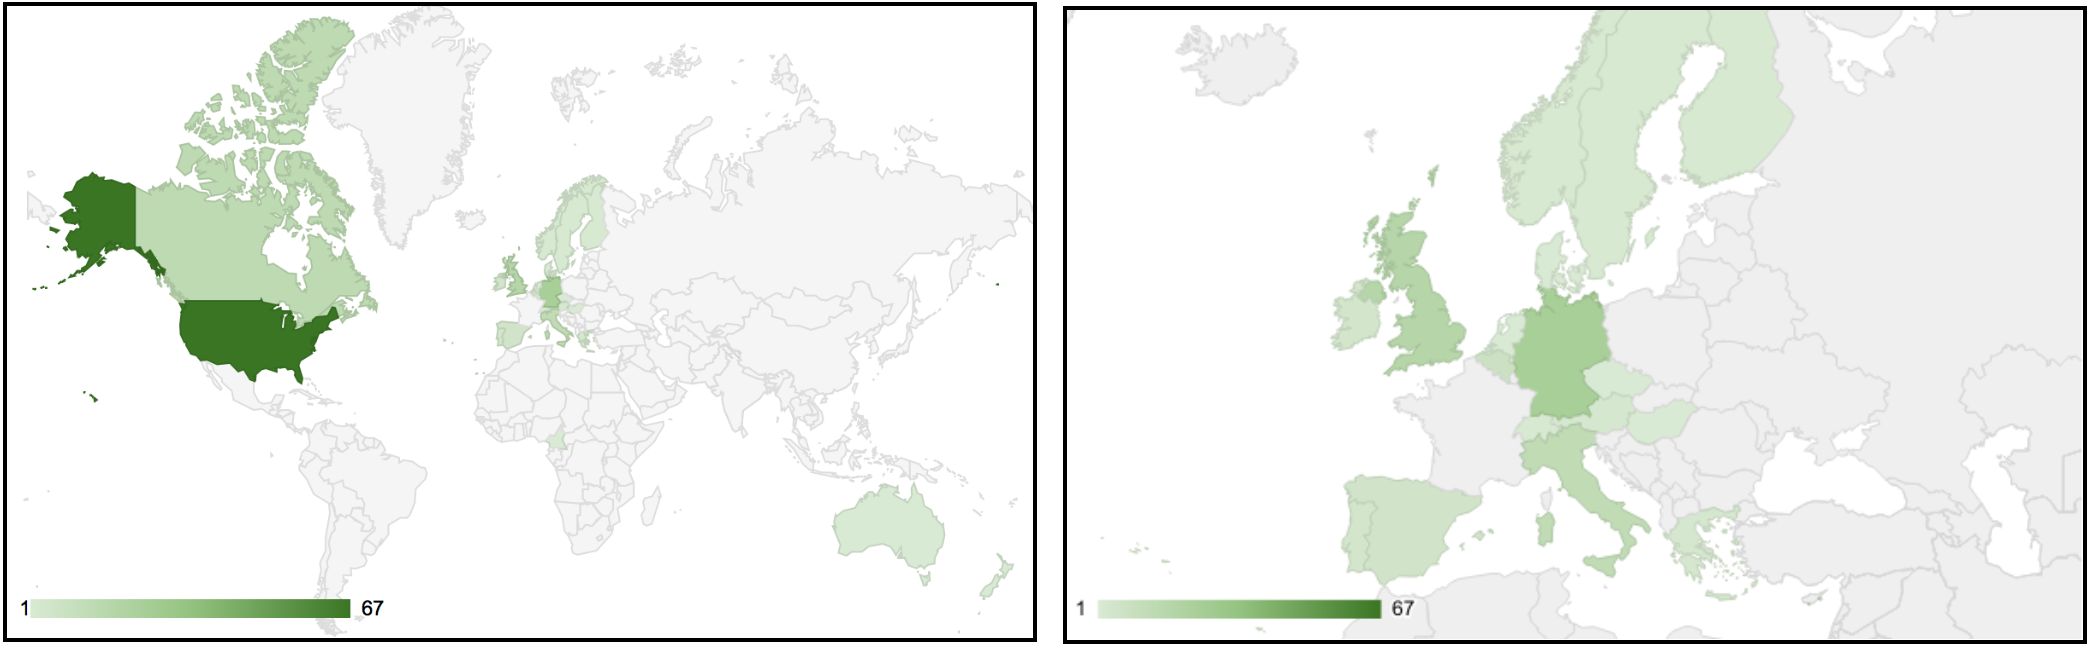
\includegraphics[width=\textwidth]{media/martinez1.png}
\caption[Demographic distribution of survey respondents (left); zooming in on distribution in Europe (right).]{Demographic distribution of survey respondents (left); zooming in on distribution in Europe (right).}
\label{demographic}
\end{figure}

As we were purposefully targeting respondents who had experience using
and/or creating digital scholarly editions in the email and social media
messages we distributed, our sample contained a marked professional
bias. Within that group, the demographic data showed a clear majority of
respondents who self-identified as digital scholarly editors and
librarians, and less participation from those who referred to themselves
as technical support (e.g. software \mbox{development} or interface design), or
from users of digital scholarly editions.\footnote{Although DSE creators
  are often also users --- and perhaps arguably even the primary target
  readership --- of other DSEs, so the roles can be fluid.} As mentioned
above, our respondent pool also contains a clear bias towards Northern
American (82 respondents, or almost 37.5\%) and European participants (106 respondents, or almost 48.5\%), with only three respondents (or just over 1\%) from the rest of the world (see Figure \ref{demographic}).\footnote{Twenty-eight out of 219 respondents did not supply sufficient information to determine their nationality.} We expected this bias, as
the field is already largely skewed toward these locations, and because
of the dissemination channels we used (Twitter, Facebook, Western
mailing lists, etc.), our personal network (which we used to send
reminders about the survey), and the fact that the survey itself, as
well as all our follow-up communication about the survey, was written in
English.

Although this bias needs be taken into account in the survey's analysis,
it does not pose an intrinsic problem for our results. As a primarily
qualitative survey, this is in essence an exploration of how the
concepts of access and accessibility are perceived in a sizable subset
of users and practitioners, and we were more interested in individual
positions and motivations than in exposing trends and making
generalizing claims about the field itself. Thus, we included responses
from participants who did not complete the survey: their opinions on the
specific questions or subsections in which they were interested still
provided us with equally valuable feedback, especially in a reflective
study like this one.

The survey was structured around a series of themes relating to aspects
of access and/or accessibility. After a demographic section (Q1-3) and a
section designed to gauge the respondent's involvement or role in the
development or publication of digital scholarly editions (Q4-6), the
survey first focused on Open Access and licensing issues (Q7-11); access
to the underlying code and software of the edition (Q12-18); cataloging
and dissemination of digital scholarly editions (Q19-21); web
accessibility (Q22-30); and inclusivity (Q31-37); before ending with a
general question about digital scholarly editions, and an inquiry
whether the respondent had any additional comments, or was open to the
possibility of a follow-up interview (Q38-42).

In the welcome page of the survey, we established a baseline vocabulary
for our respondents by providing short definitions of some of the most
important concepts that we used throughout the survey. These were:
\begin{quote}
\textbf{Access:} \emph{the ease or difficulty of users finding and interacting with digital scholarly editions.}\par
\textbf{Inclusivity:} \emph{the focus on
representing and including people/groups who would otherwise be
marginalized.}\par
\textbf{Web Accessibility:} \emph{the design of digital interfaces for use by people with (in)visible disabilities.}\par
\textbf{Digital Scholarly Edition:} Our
definition includes (but is not limited to) an amalgamation and
paraphrasing of two definitions offered by Patrick Sahle (\citeyear{sahle_catalog_2008} and
\citeyear{sahle_what_2016}): \emph{A digital scholarly edition is an information resource
which offers a critical representation of (normally) historical
documents or texts and which is guided by a digital paradigm in its
theory, method and
practice.}
\end{quote}
Since we were primarily interested in the respondents' individual
perspectives, we encouraged them to provide their own definitions for
these concepts at distinct points in the survey (Q7, Q31, Q22, and Q38,
respectively). The fact that many of these personal definitions deviated
strongly from our own (and from one another) confirmed our premise that
access is a layered concept that is used to mean different things in
different contexts. As will be elaborated below, these differentiations
proved to be fundamental points of discussion, particularly in relation
to web accessibility, and must be taken into consideration for the
analysis of the survey's results.


\section*{Challenging the concepts of access in Digital Scholarly
Editing}

\subsection{Dissemination}

We begin this discussion by approaching access from the broadest
possible sense, which corresponds to the definition we gave at the start
of our survey. Access to a digital scholarly edition in the sense of
interacting with the edition is inherently linked to its
discoverability. The challenge of discoverability extends far beyond the
realm of digital scholarly editions alone; it is an issue affecting
digital scholarly outputs throughout the academic world. As the Ithaka
S+R research team observed: ``Digital projects on campuses live
everywhere! This extreme decentralization adversely affects their
discoverability. {[}. . .{]} There is often no single place for users to
find digital projects and some projects can too easily slip from view'' \citep[4]{maron_sustaining_2013}. The digital ecosystem of scholarship
continues to increase in size and complexity, while patterns of
information retrieval also morph and mutate, which makes the effective
dissemination of digital scholarly editions extremely challenging,
particularly for those editors who are making the transition from print
to digital editing, and for new students in the discipline.

The purpose of the dissemination section of the survey was to gain
insight into the means through which respondents make their digital
scholarly editions known to users. This also highlights the extent to
which the respondents are aware of the various ways that users discover
and use their resources. We opened this section by asking how the DSEs
with which respondents were involved were disseminated and marketed
(Q19). We provided a list of options and asked respondents to choose any
or all that applied in their case, and to specify if they used another
method not in the list. Interestingly, despite the digital nature of
their projects, it was evident from the results that traditional methods
of promoting editions remain the most prevalent approaches. By
``traditional'' we mean methods that existed in the analogue pre-digital
turn. The top four results from the list were all in this category: word
of mouth (67\%), conference presentations (67\%), citations in articles
written by the team (64\%), and citations by others (58\%). The two most
used digital methods of promoting DSEs were social media (57\%) and
Listservs (42\%).

A more interesting, and perhaps slightly concerning, observation from
the results was the relatively less commonplace usage of existing
digital catalogues to make digital scholarly editions discoverable. Only
29\% of those who responded chose the option of ``through catalogues in
one or more memory institutions''. Essentially, if students and
researchers were to rely on institutional or aggregated catalogues (e.g.
NINES or Europeana) as principal finding aids, they may struggle to find
digital scholarly editions that even originated at their own
institutions. While some digital scholarly editions are created in
collaboration with librarians or archivists, there are many created by
scholars working independently from such institutions that may benefit
greatly from the expertise of LIS professionals in order to make the
editions more findable through effective cataloguing. One of the biggest
challenges faced in that domain of digital scholarly editions is
classification, a concern which, in the words of Elena Pierazzo
``pervades digital scholarship'' (\citeyear[6]{pierazzo_digital_2015}). The difficulty for digital
textual scholars to find common ground about whether a digital project should
be deemed a digital edition, library or archive is not merely a semantic
squabble, but a practical bibliographic issue with substantial impact on
discoverability, and thereby dissemination in general.\footnote{See Kenneth
  \citealt{price_edition_2009} for a detailed discussion of this topic.}

The two most prevalent catalogues of digital scholarly editions, one
created by Patrick \citet{sahle_what_2016} and the other by Greta \citet{franzini_catalogue_2016},
were among the lowest scoring results on the list provided at 16\% and
12\% respectively (a further 12\% of respondents found their editions in
other catalogues). Some respondents commented that they had never heard
of the two resources, while others replied that they now intended to
ensure their digital scholarly editions would be cataloged there in
future. In Q20 we asked respondents if they were satisfied with the
dissemination and marketing of their edition(s). Of the 91 responses we
received, 41 responded in the affirmative, while 26 said they were not
satisfied (the remaining 24 gave more ambiguous answers). Opinions on
who should be responsible for the dissemination of a digital scholarly
edition are often varied and this is clear from the respondents'
comments. In a print paradigm this is much clearer, as publishers have a
well-established role in the marketing and distribution of printed
editions in much the same way that libraries have a clear remit to
catalogue them. The digital avenues of distribution have blurred those
lines, as the distinct role of publisher has all but disappeared in a
digital context. It remains unclear whose responsibility it is to take
on this marketing and distribution role. One respondent put it quite
succinctly when they said: ``{[}N{]}o one knows whose task it is to
market digital scholarly editions'' (R116).\footnote{R+number is used to
  anonymize respondents, and refers to respondent number to the overall
  survey.}

The responses we received indicate that there remains a need for further
reflection and discussion in the field about how digital scholarly
editions are disseminated to and made findable by users. Aside from the
ambiguity surrounding how roles and responsibilities in this area should
be assigned, there is also a general need for increased awareness among
the creators of digital scholarly editions regarding the variety of
dissemination channels at their disposal as well as for information
about retrieval habits of users. These needs are not surprising, given
that many of these issues are new to editors who previously relied on
print-based publishers to tackle distribution, and for whom papers and
presentations were the primary avenues of knowledge-sharing. While
classification and cataloguing challenges will not be solved by the
digital scholarly editing community alone, they cannot be neglected, and
are only likely to improve through deeper and more critical
collaboration with academics in other disciplines, with archivists and
with librarians.

\subsection{Open Access and licensing
issues}

Moving from a broader conception of discoverability, we now explore the
definition of access most often used in the field: that of Open Access
(OA) and its inextricable link to licensing issues. Coined in 2002 by
the Budapest Open Access Initiative to mean ``the free and unrestricted
online availability'' of published and pre-published research \citep{chan_read_2002}, OA builds on a longstanding tradition of Open Source (OS)
software development on the one hand and on \emph{ad hoc} practices of academic
self-archiving on the other. Although the term is now commonly used in
relation to scholarly communication and digital scholarship \citep{suber_open_2012,eve_open_2014}, there are still diverging interpretations of OA in the field
of digital scholarly editing as well as a confusing number of coexisting
standards and strategies for licensing scholarly content \citep[440]{sichani_beyond_2017}. Given that practitioners of digital textual scholarship and
digital scholarly editing are working particularly with historical and
archival-based textual material, and are therefore likely to be
confronted with licensing restrictions, this section is intended to
offer some insight into the developments of Open Access in these
communities of practice.

Rather than documenting what kind of licensing restrictions or copyright
status digital scholarly editions typically have, however, the licensing
section maps our respondents' awareness regarding issues and levels of
Open Access.\footnote{For more information on these issues, see \citealt{dillen_digital_2016} and \citealt{sichani_refining_2017}.} Because we wanted to assess the
community's engagement with the topic, we designed this section with two
tracks of questions to the subjects of OA and licensing that actively
avoided guided replies. To assess the importance of licensing issues
with regard to digital scholarly editions within our sample, we kept all
questions in this section optional.\footnote{We also tried to keep the
  phrasing of the questions as neutral as possible and strategically
  combined a series of closed and open-ended questions, offering
  respondents the option to elaborate on their perspective in a comment
  box.} The fact that just over two-thirds of all respondents (149 out
of 219) answered these optional questions and provided useful comments
was a clear indication that these are indeed issues important to the
digital scholarly editing community.

\begin{figure}[!ht]
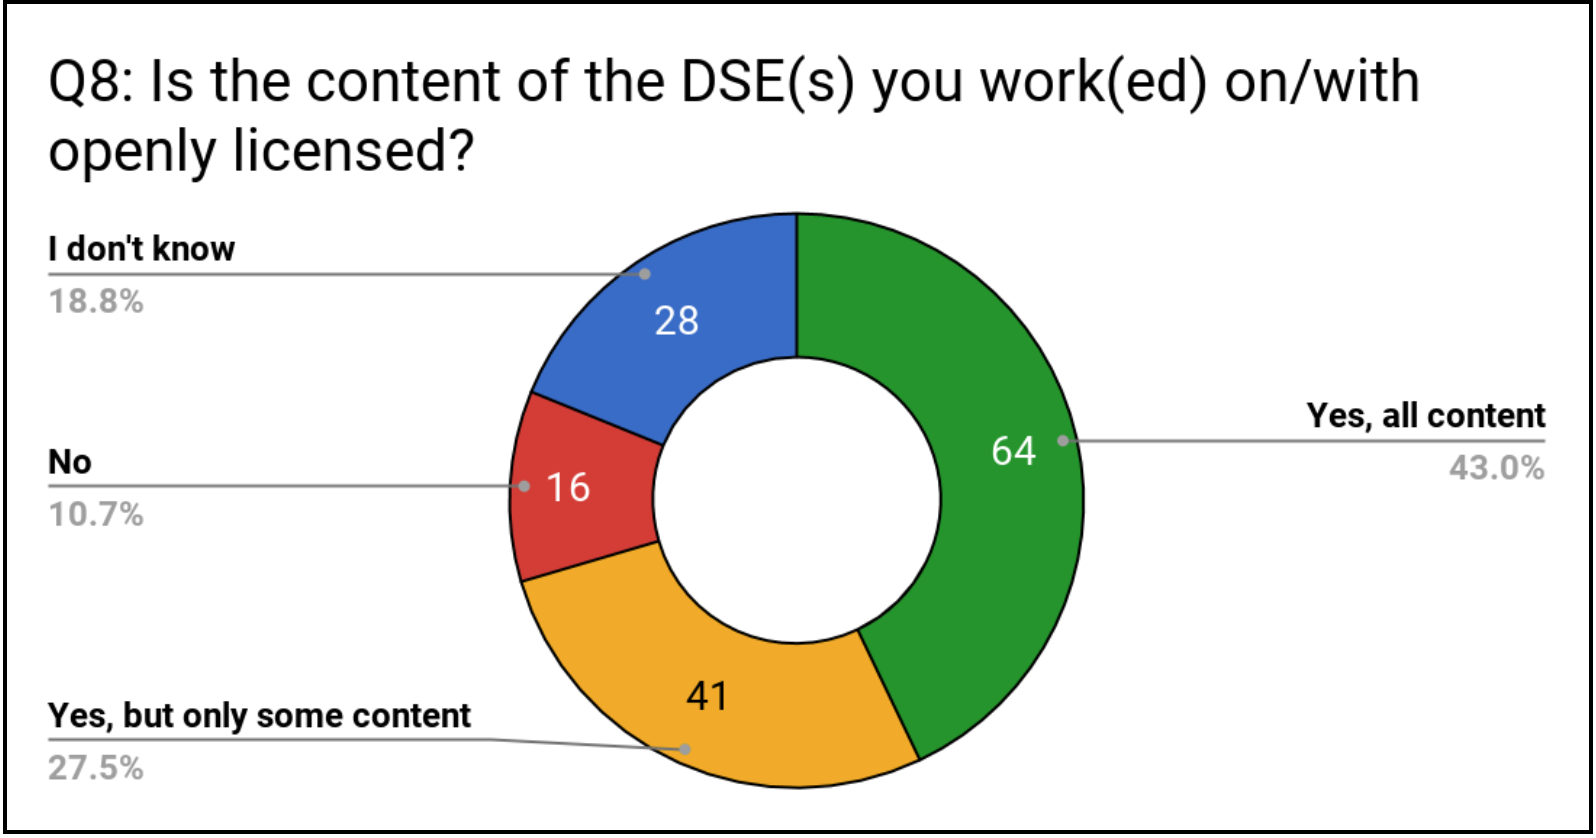
\includegraphics[width=\textwidth]{media/martinez2.png}
\caption{Response breakdown of Q8.}
\label{q8}
\end{figure}

We began by asking participants whether the content of the digital
scholarly edition(s) on which they work(ed) (as creators), or with (as
users), is openly licensed (Q8). The purpose of this question was
twofold: (a) to indicate awareness of the licensing and OA landscape in
general and (b) to provide crucial data of the specific licensing status
of their DSEs. As Figure \ref{q8} shows, while the majority of respondents
(105, or 70\%) answered that the content is openly licensed at various
levels, a substantial amount of people indicated that they were not
aware of the licensing status of their work at all. Useful insights from
the comments mentioned various barriers to OA such as rights clearance
(for mainly twentieth-century source materials) or partner agreements'
provisions. Others indicated that they distinguished between different
licenses or reuse statuses for different data types (e.g. texts vs.
images) within the same edition. The issue of open documentation
alongside CC licensing was also raised several times: ``We're using
Creative Commons licences, which seems sufficient. Of course, explicit
documentation about re/use conditions wouldn't harm'' (R112).

To deepen our understanding of the community's awareness of licensing
issues further, we asked respondents to provide the name of the license
under which their digital scholarly edition is published (Q9). This
question asked for open-text responses to allow people to be as specific
or general as they wished, while allowing us to assess their
understanding of licensing standards and protocols. To frame the
question, we gave respondents a concrete example (``e.g. CC-BY-SA-4.0 or
similar''). The Creative Commons licensing scheme was the most popular,
with respondents offering a number of variations on the CC license as
well as referencing other licensing schemes that were better suited to
different types of scholarly outputs (e.g. content vs. code).

After mapping respondents' awareness of licensing for digital scholarly
editions, we asked about current institutional policies on Open Access.
While setting up and adopting OA institutional policies for various
scholarly outputs such as digital scholarly editions may help enforce
licensing considerations, making OA a requirement could impede a more
active engagement and understanding of OA based on a conscious scholarly
choice: we don't always understand or support a regulation we're forced
to follow. Furthermore, it is important to note that OA regulations tend
to create tensions between institutional policies and funders' agendas,
when we want to assess the socio-economic and scholarly questions that
are currently at stake. By asking two distinct questions on
institutional and funders' provision towards OA (Q10 and Q11), we wanted
to imply a clear distinction between the two and, more importantly, see
if any gaps or grey areas exist regarding OA implementation, especially
in the case of complex digital scholarly outputs. This last aspect is
especially relevant in relation to digital scholarly editions, as
stakeholders' guidelines vary widely in terms of openness,
comprehensiveness, and style as well as in how they conceptualize the
multitude of research outputs and their related licensing status. To
leave room for this issue, we provided our respondents with a comment
box where they were encouraged to list specific licensing regulations
pertaining to ``the edition itself, the underlying code, metadata,
scholarly outputs or manuals resulting from the digital scholarly
edition''. An interesting response also describes Open Source tools and
services as part of the institutional compliance of the digital
scholarly editing project to Open Access:

\begin{quote}
I have licensed my two first digital projects with Creative Commons
Attribution Non-Commercial 3.0. Most of my work is funded by public
bodies so it has to be freely available for reuse. {[}. . .{]} The data
(XML) is all available on Github. I have used EVT2 to publish my digital
edition of the {[}redacted{]} which is a free open source tool. In
regard of {[}redacted{]}, we are using Kiln with publication purposes --
this is again all free and available online. In addition to Open Access,
I have documented my editorial criteria on Github and also written
extensively about the whole process in a number of articles and papers.
\begin{flushright}
(R13)
\end{flushright}
\end{quote}

The majority of our respondents' institutions do not require open
licensing for research outputs (57 responses, or 38\%), in contrast to a
relatively small number of institutions where open licensing is
mandatory (27 responses, or 18\%). It should be noted that a substantial
amount of respondents indicated they were simply not aware of their
institution's Open Access policy for digital scholarly editing projects
(40 out of 149 respondents, or almost 27\%). As for the funders' OA
requirements (Q11), the results were quite evenly distributed among
respondents that indicated their funders \emph{do} require open
licensing (30, or 20\%), those that \emph{do} \emph{not} (32, or
21.5\%), and respondents who indicated that their project did not fall
under a funding scheme at all, allowing them to make a more conscious
decision when it comes to licensing their digital scholarly edition
(also 32 respondents).

To conclude, the answers we gathered in this section underlined the
importance of Open Access for digital scholarly editions, the growing
awareness of the community about licensing and reuse issues, and the
diverse stakeholders' takes on establishing OA policies. As issues of
licensing are usually linked to copyright regulations, e.g. for
historical documents, it is often difficult to balance the scholarly
will and/or commitment to an OA ethos with compliance to external legal
and financial regulations. On the other hand, OA as a scholarly movement
is about inventing financial, legal, intellectual and administrative
models in order to redistribute the power of knowledge; what we are
observing from this section is that the digital editing community is
actively exploring ways to make this happen by balancing the restricted
access or reuse of copyrighted material with open documentation or by
adopting Open Source tools and development frameworks.

\subsection{Access to the code}

With Open Access being an emerging topic in digital textual scholarship,
it is worthwhile to take a closer look at what we understand by the
\emph{content} of digital scholarly editions. In general, content
usually means the source material in some digital form (e.g. digital
facsimiles and transcriptions of the source text). To be sure, the
capacity of digital editions to provide access to primary sources has
always been a major selling point of the digital medium. And, as
Lavagnino noted, a digital edition differs from a digital library
because it contains a fair amount of scholarship in addition to digital
reproductions of existing texts \citep[63]{lavagnino_access_2009}.\footnote{We can
  even make the argument that digital reproductions are a product of
  scholarship as well. At the very least they are equally subject to
  interpretations of the specialist that makes them. This ranges from
  technological factors like lighting and camera settings to a choice
  about what elements to capture and what not. In short, digital
  facsimiles are always an approximation of the source document.} It has
been generally acknowledged and accepted that transcriptions, for
instance, convey a scholarly interpretation rather than objective
findings. Incidentally, this holds true for both print and digital
transcriptions.\footnote{In 1971 Hans Zeller argued that scholarly
  editing is ``ineluctably'' subjective, which isn't a bad thing in
  itself; in fact, the scholar's insights and knowledgeable
  interpretation can help others understand the text \citep[22]{zeller_befund_1971}.
  It's more important, therefore, that editors clearly communicate about
  their decisions and methodology than that they strive towards an
  unattainable standard of objectivity (see also \citealt[41]{bleeker_mapping_2017}).}
Arguably, though, another key component of the edition's content is its
code base. Code, in the broadest sense of the word, provides users with
various tools to access and examine the source materials. It seems
evident, therefore, that an edition's code base should be made available
for critical evaluation too \citep{bodard_open_2009}. All the more so if
we consider that a digital scholarly edition makes use of tools that
transform and manipulate its source materials for the benefit of the
user. How to critically assess an edition's code base, however, has only
become a point of concern in recent years.

As with every topic in the article, a code base is an intricate issue
that needs more context. We will therefore start by asking what the code
of a digital edition is exactly, before we go on to discuss the current
approaches to providing access to it. So what do we mean when we talk
about the code of an edition? In and of itself, ``code'' appears to be a
term as broad as the term ``access'' --- and as diversely defined. In the
context of a digital scholarly edition, we can distinguish source code
from other underlying material. Source code is understood to be ``a
blueprint for a {[}computer{]} program that can be executed'', meaning
something written in a formal language that is interpreted by a computer
and results in executable software \citep[121]{van_zundert_code_2017}. ``Other underlying material'' constitutes a more ephemeral
category and includes (but is not limited to) digital transcriptions, a
database or content management system, associated style sheets and
schemas, a graphical user interface, and a search engine. In addition to
the source code and the underlying material, an edition can make use of
integrated existing software like a collation engine or a data
visualization tool to process the text files. This could be software
that is specifically developed for the edition, software developed by
external, independent parties, but tweaked to match the research
purposes of the edition, or Open Source software that is integrated
unaltered. To date, there has been little agreement on what of this
amalgam of databases, software, stylesheets, query functions and
transcriptions makes up the code of the edition. Everything together or
just a selection? And if the latter, on what grounds is the selection
made?

In this respect, another interesting perspective is that of the
archivists and librarians who take charge of preserving digital
editions. What aspects do they consider as essential parts of a digital
scholarly edition? The Dutch digital archiving institute Data Archiving
and Networking Services (DANS) takes a universal approach and aims to
store as much data as possible.\footnote{\href{https://dans.knaw.nl/en/about/organisation-and-policy/policy-and-strategy/preservation-plan-data-archiving-and-networked-services-dans-1}{https://dans.knaw.nl/en/about/organisation-and-policy/policy-and-strategy/ preservation-plan-data-archiving-and-networked-services-dans-1}, accessed 30 June 2019.} The group recognizes the risk of digital files becoming obsolete as
hardware changes, and while they lament their lack of means to preserve
hardware, they intend to store at least information about the digital
environment and the hardware required to access the data set (DANS
Preservation Policy version 1.0, 2018). Another important aspect that
certainly influences how digital editors feel about the code of a
digital scholarly edition is whether or not they consider code to have a
scholarly quality. The editing community may agree that a digital
transcription represents an interpretation, but less attention has been
paid to the question of whether the edition's code also constitutes a
form of scholarship. Users often attribute a neutral or objective
quality to software, but software that is used to query, process, or
analyse the edition's data is often constructed based on certain
scholarly assumptions and decisions. An Open Source collation engine
like CollateX, for example, reflects the prevalent scholarly
understanding of text collation and makes, \emph{inter alia}, certain
assumptions about what constitutes a token and when two tokens form a
match.\footnote{CollateX
  (\href{https://collatex.net/}{{https://collatex.net/}}) is developed
  within the framework of the Interedition project (2007-2011) and
  maintained at the Digital Infrastructure department of the Humanities
  Cluster at the Huygens Institute in Amsterdam.} The same applies to graphical interfaces that
inevitably steer a user's gaze and influence how the edition's data is
accessed and perceived.\footnote{This topic was the theme of a symposium
  on scholarly editions and interface design, ``Digital Scholarly
  Editions as Interfaces'', at the Centre for Information Modelling in
  Graz, Austria (23-24 September 2016). The contributions to this
  symposium are bundled in a special volume of \emph{Schriften der
  Institut für Dokumentologie und Editorik} \citep{bleier_digital_2018}.}

Still, the variety of digital editions, representative of a field that
continues to develop, makes it difficult to come to any conclusive
definition of a code base. For that reason we have refrained from
adopting a narrow definition of ``code'' in the survey to leave room for
idiosyncratic, project-specific interpretations. One disadvantage of
such a broad definition is that not all respondents understood what was
meant by ``code'' which was for some an incentive to skip the questions
(e.g. Q15, R185; Q16, R120; Q17, R176). Others, on the contrary, decided
to leave a lengthy and detailed response, listing every program their
project uses. These wide-ranging and diverse responses are difficult to
summarize and do not exactly help with narrowing down and refining the
definition of code. An important benefit, however, is that this survey
provides us with perhaps the most comprehensive overview of current
digital editorial practices. Indeed, when taking a closer look at the
commentary in response to Q12 and Q13 (``what type of software does your edition
use?'') we see a highly diverse understanding of software. Respondents
list specific editorial tools like eXist DB and CollateX, but also more
general tools like git version control, Google Sheets, and MS Office
suite. In addition to tools, standards like TEI (P5) (Text Encoding
Initiative Proposal 5), HTML (Hypertext Markup Language) or CSS
(Cascading Style Sheets) appear to be considered part of software as
well.

As mentioned above, editorial strategies geared towards providing
suitable and sufficient access to code are affected by how the concept
of code is defined. In other words, if software isn't considered to be
part of the scholarly content of an edition, editors are less inclined
to put any effort into making its source code accessible. In the context
of the survey, we've understood access to code as the possibility for
end-users to see which software is used and how the scripts and tools
together manipulate the content of a digital scholarly
edition.\footnote{This definition was inspired by the Modern Language
  Association's 2016 publication on digital scholarly editions, which
  states the importance of documenting how the edition was created,
  including processes that otherwise remain invisible like algorithms,
  data structures and constraints \citep[7]{mla_modern_2016}.} This definition
adheres to the idea that knowledge is inseparable from the way it is
made.\footnote{A statement recently repeated by Willard McCarty in his
  keynote lecture at the international conference on Computational
  Methods for Literary Historical Textual Scholarship \citep{mccarty_what_2018}.} A similar sentiment was expressed by survey
respondents who overwhelmingly responded positively when asked if they
considered it important to share information about the technical aspects
of the edition and the underlying data (Q18). The responses underline
that the question isn't so much ``\emph{should} the code be made
accessible'', but rather ``\emph{how} should the code be made accessible?'' This question is strongly related
to the issue of education and training. In her talk at the 2016
conference of the European Society for Textual Scholarship, Elena
Pierazzo rightly noted that it's unfeasible to expect scholarly editors
to be experts in textual scholarship, information modeling, data
structures, APIs and interface design.\footnote{In a joint talk with
  Susan Schreibman and Franz Fischer entitled ``DiXiT: Research,
  Training, and Networking in the Field of Digital Editing'' at Digital
  Scholarly Editing: Theory, Practice, Methods, Thirteenth Annual
  Conference of the European Society for Textual Scholarship, Antwerp, 6
  October 2016.} Training in digital scholarly editing is a key concern,
and the amount of institutional programs and online training material
that is available has increased in the last decade. Still, those new to
the field of digital editing (whether they are early career scholars or
senior scholars making the transition from print to digital) may not
necessarily know where to look for those materials or even where to
start.\footnote{Good starting points are the website of the DiXiT
  project, which contains all materials of the training camps and
  workshops
  (\href{http://dixit.uni-koeln.de/}{{http://dixit.uni-koeln.de/}},
  maintained by the University of Cologne), the NEH Institute ``Make Your
  Edition''
  (\href{https://pittsburgh-neh-institute.github.io/Institute-Materials-2017/}{{https://pittsburgh-neh-institute.github.io/Institute-Materials-2017/}})
  and the personal website of David J. Birnbaum of the University of
  Pittsburgh (\href{http://obdurodon.org/}{{http://obdurodon.org}}). All
  links accessed on 30 June 2019.} Based on our experiences within
DiXiT, we confirm that expecting digital editors to be ``super editors''
is not only unrealistic but also unnecessary \citep{pierazzo_digital_2016}. A more
realistic approach would be for editors to have a conceptual
understanding of text modelling and, importantly, to be able to
collaborate and communicate effectively with specialists in information
science.

Respondents also confirmed the observation made in the introduction to
this article: most editors consider access to code important, but
opinion as to how to share code remains disparate. For instance, digital
scholarly editors could provide extensive technical documentation or
content themselves by providing a link to an online GitHub repository
that contains all scripts of their editions. Without some commentary or
annotation, however, these scripts would be difficult if not impossible
to read for the uninitiated. We can break this issue down in at least
three key aspects, the first one naturally having to do with what is
defined as the edition's code. Is it the complete set of scripts, the
interface(s), and software packages taken together, or a selection
thereof? Second, there are different degrees of access to the code.
Someone who has a broad and inclusive understanding of ``code'' may
still consider it unnecessary to make the entire set available to the
end-user. For example, the technical criteria for \emph{RIDE}, the
review journal for digital scholarly editions, only asks about
availability of what they call ``basic data'' --- XML transcriptions of the
source texts --- and not so much the operations on those source
texts.\footnote{The \emph{RIDE} questionnaire focuses on another key
  issue: the reusability of the edition's data.} Third, if an edition
makes use of tools developed by external parties, it may be challenging
for the team to provide detailed insight into how these tools operate.
This point is particularly relevant, as over 70\% of our respondents
indicated that they make use of existing open source software (Q12). One
could argue that, in this case, the responsibility lies not with the
editorial team, but with the tool developers. Is it not reasonable to
assume that creators of digital scholarly editions have made an informed
choice regarding these tools? That they are aware of how the edition's
data is manipulated and that they are able to justify their choices? In
reality, again, editorial practices vary. Several respondents indicated
that providing access to the code was a goal at the outset of their
projects, but was never (fully) realized: one respondent commented that
``associated XML files, as well as documentation concerning their markup
and associated technical systems{[},{]} was supposed to be made public
but was never done'' (Q16, R196). Others admit that they have no idea
whether or not any of the underlying code (transcriptions or scripts)
are available. Still, with the majority of answers being favorable
towards open repositories like GitHub for storing datasets, it seems
that the real challenge lies not in the general mentality but rather in
the methodology.\footnote{As a final point, it is worth taking a closer
  look at reasons for not providing access to the code of a DSE. Answers
  range from straightforward (the editors do not know how the code
  works) to complex (part of the code is licensed), from principled (the
  code is considered as subservient to or less important than the source
  material) to aesthetic (the code is considered too ugly to publish).}
We therefore strongly recommend any future work to focus on establishing
standards for a technical rationale of digital scholarly editions. In
particular, we see value in (1) the development of guidelines for
communicating the data transformations produced by tools and software
used; and (2) providing clear instructions about the possibilities to
(re)use the scholarly data set. Such recommendations are tightly
intertwined with the pedagogical issues outlined above.

\subsection{Web accessibility and usability}

Having broached the subject of code and accessibility to the entire
digital scholarly edition environment itself rather than its contents
alone, we wanted to examine the concept through the lens of web and
software development. In this context, the term accessibility has a very
specific meaning, where it refers to the adoption of strategies that
make the application accessible to all users --- including those with
(in)visible disabilities. George H. Williams lamented the fact that
although ``{[}o{]}ver the last decades, scholars have developed
standards for how best to create, organize, present, and preserve
digital information'' for future generations, ``the needs of people with
disabilities'' have largely been neglected in this pursuit (2012, 202).
Indeed, especially in the field of digital scholarly editing,
discussions regarding different user needs typically refer to those with
non-academic backgrounds (\citealt[93]{apollon_digital_2014}; \citealt[151]{pierazzo_digital_2015})
rather than to users with (in)visible disabilities. In addition, as two
major points of reference in the field, neither Sahle's \citeyearpar{sahle_what_2016} nor
Franzini's \citeyearpar{franzini_catalogue_2016} catalogues mention accessibility in their respective
lists of criteria for digital scholarly editions. This suggests that
otherwise widely adopted standards such as @alt texts for links and
images, consistent use of header tags, legibility of fonts, attentive
use of colors and contrast, etc. are not sufficiently acknowledged or
adopted in the field.\footnote{This shortcoming becomes particularly
  poignant when we take into account that the digital medium gives the
  DSE the capacity to be more accessible than its print predecessor ---
  and perhaps especially so when the DSE is published on the Web, a
  medium that ``is fundamentally designed to work for all people,
  whatever their hardware, software, language, location, or ability'',
  as it ``removes barriers to communication and interaction that many
  people face in the physical world'' \citep{w3c_accessibility_2018}.} In the web
accessibility section of our survey, we wanted to test this hypothesis,
while also gauging the community's perspective about making
accessibility a prevailing concern for digital scholarly editions.

The first goal of the web accessibility section was to map respondents'
awareness of relevant accessibility guidelines by practitioners in the
field. To this end, we asked our respondents whether the digital
scholarly editions on which they worked adhered to any established web
accessibility guidelines (Q23).\footnote{By answering either `yes' or
  `no' to this question, respondents indicated that they were at least
  aware of the efforts their development team were making in this
  respect, while answering `don't know' indicated that they were not. An
  `other' option with comment box was also provided for people to whom
  the question did not apply (e.g. because they were not involved in the
  development of a DSE) or for those who wanted to provide a more
  nuanced answer. Delving deeper into the `other' category allowed us to
  attribute a few more answers to the other three categories, and
  suggested that there was a substantial part of digital scholarly
  editions that provide partial compliance to web accessibility
  standards.} In total, 75 respondents (64.5\%) indicated that they were
at least aware of the efforts their development team were making in this
respect (with 31 indicating compliance, 9 indicating partial compliance,
and 35 indicating non-compliance to web accessibility standards), with
37 (31\%) indicating they were not aware. These results suggest that
awareness of web accessibility practices is still an issue in digital
scholarly editing, and that most editions do not actively (or only
partially) comply to relevant standards. Cross-referencing these results
with respondents' demographic data, however, revealed an interesting
geographical divide (see Figure \ref{q23}).\footnote{The nine respondents that are not included in these two graphs either did not enter usable demographic information in the survey or were situated on a continent that was underrepresented in our survey.} When we just look at ``yes'' and
``no'' answers, we see that for Europe ``no'' responses outrank ``yes''
almost two to one; while in Northern America the answers are reversed,
with ``yes'' responses outranking ``no'' almost three to one. This
suggests that web accessibility practices in digital scholarly editions
are much more common in Northern America than in Europe. This divide
makes sense when we realize that both the USA and Canada have laws or
policies in place requiring web accessibility for digital output of
publicly funded projects and that this is not the case for many European
countries \citep[205]{williams_disability_2012}.

\renewcommand*{\thefootnote}{\fnsymbol{footnote}}
\begin{figure}[p!]
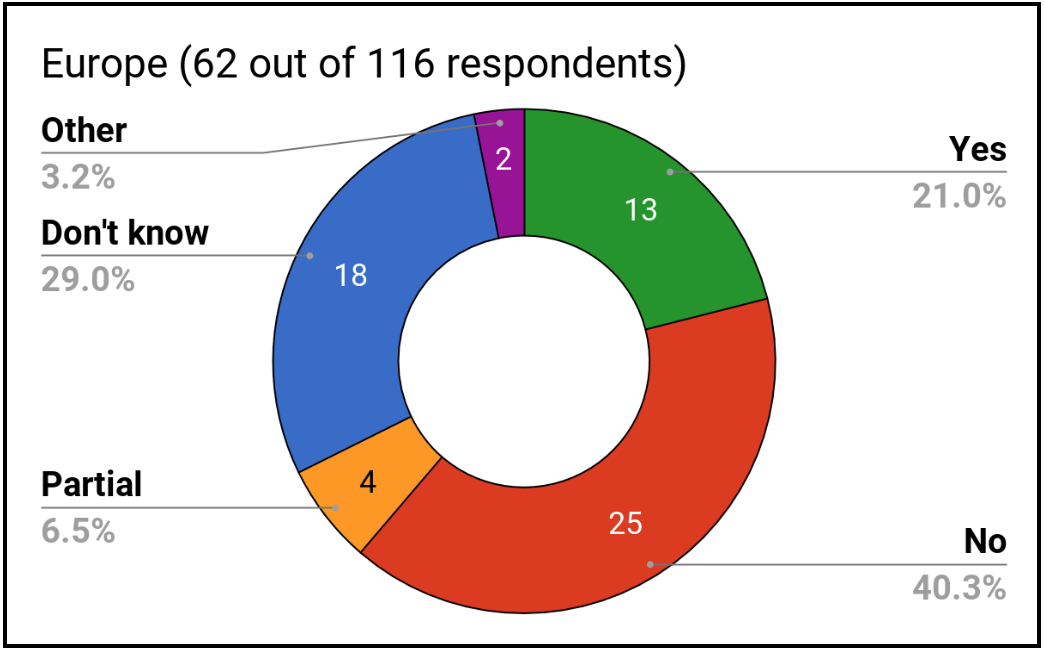
\includegraphics[width=\textwidth]{media/martinez3a.png}\\
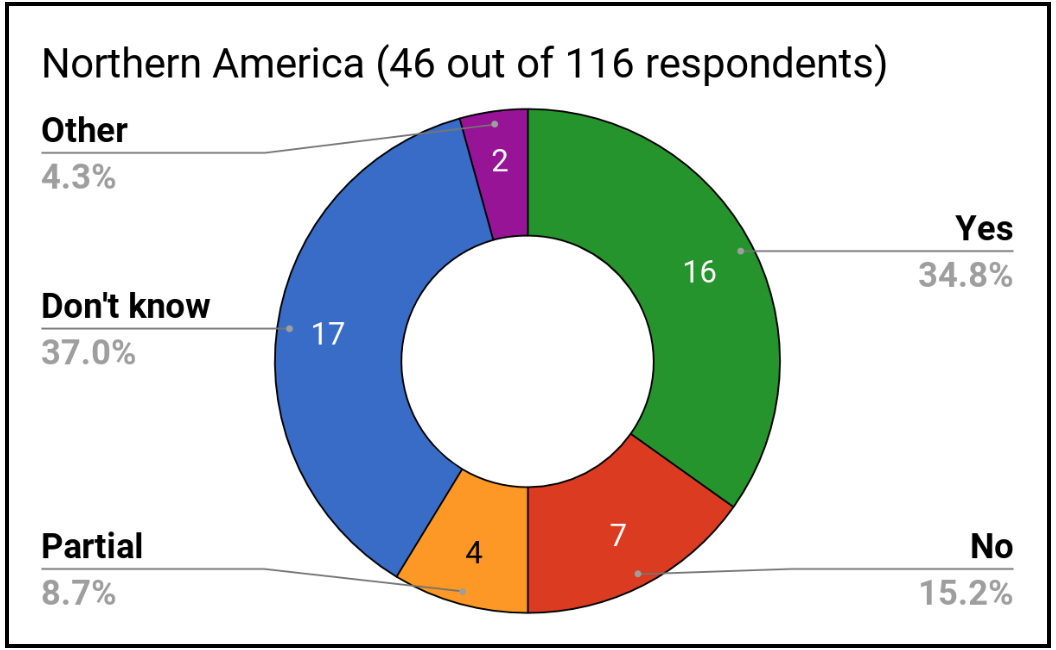
\includegraphics[width=\textwidth]{media/martinez3b.png}
\caption[Responses of Q23 ``Do(es) your digital edition(s) adhere to any established web accessibility guideline(s)?'', contrasting answers from European respondents (left) with those of
Northern American (right) respondents.]{Responses of Q23 ``Do(es) your digital edition(s) adhere to any established web accessibility guideline(s)?'', contrasting answers from European respondents (left) with those of
Northern American (right) respondents.}
\label{q23}
\end{figure}
\renewcommand*{\thefootnote}{\arabic{footnote}}

For editing projects that \emph{did} provide web accessibility options,
we wanted to know what kind of options these were (Q25). This was an
optional open-ended question to encourage respondents to share any web
accessible option that sprang to mind. Sadly, the response rate to this
question was low (with only 23 usable answers).\footnote{We received a
  total of 48 answers, 19 of which (i.e. almost 40\%) were disqualified
  because respondents did not mention measures that were taken to make
  the edition more accessible. In addition, six more respondents
  referred to standards, platforms, tools and/or validators they had
  used, rather than mentioning specific accessibility options --- leaving
  the total at 23.} We grouped answers into different categories, to
determine what kind of measures digital scholarly editing teams were
focusing on --- or, failing that, at least those of which our respondents
were aware. These categories were based on the four ``principles of
accessibility'' that the W3C's Web Content Accessibility Guidelines
(WCAG) are organized around:\footnote{Specifically, we used version 2.1
  of the guidelines \citep[see][]{w3c_web_2018}.}
for web content to be accessible, it needs to be ``perceivable''
(presented in a way users with different abilities can perceive);
``operable'' (presented in a way user with different abilities can work
with); ``understandable'' (presented in a way users with different
abilities can understand); and ``robust'' (presented in a well-formed
environment so that it can be interpreted and used by different agents
such as assistive technologies) \citep{w3c_introduction_2018}.\footnote{For
  more elaborate definitions of these terms, please refer to \citet{w3c_introduction_2018}.}
As respondents were free to list as many options as they liked, it was
possible for individual responses to be tagged with more than one of
these categories.

\begin{figure}[h!]
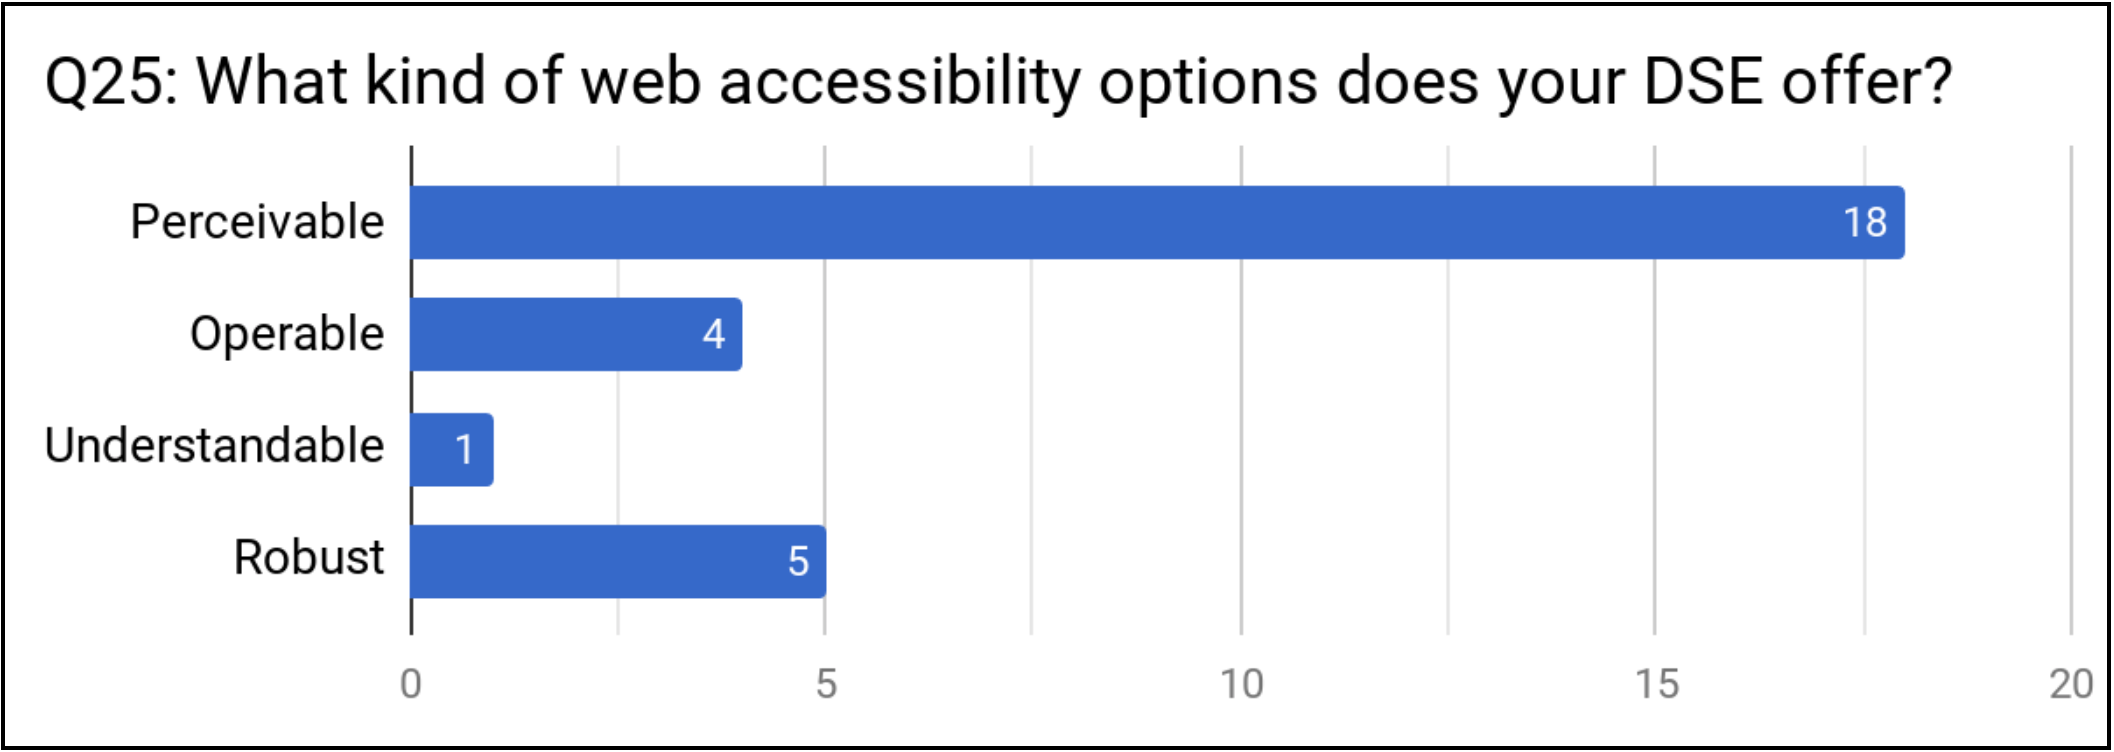
\includegraphics[width=\textwidth]{media/martinez4.png}
\caption{Classification of the accessibility options offered in
Q25 in relation to the different WCAG principles.}
\label{q25}
\end{figure}

As Figure \ref{q25} indicates, most responses focused on perceivability,
including ``text alternatives'' (e.g. careful description of images so
that they can be perceived by the visually impaired), careful use of
color, contrast, and visual presentation (e.g. using more legible
fonts), providing options for resizing the text, and making the content
adaptable to the display (responsivity). The second largest category,
robustness, focused on the structural integrity of HTML output and/or
explicit screen reader testing. In the operability category, then, all
four responses mentioned keyboard accessibility (making content
accessible through the keyboard rather than with a mouse pointer).
Finally, the one respondent that discussed understandability referred to
catering to different reading levels. It should be noted that out of the
23 usable responses, only four were given more than one tag and no
response was given more than two.\footnote{Two respondents mentioned
  measures that improved both the edition's operability and robustness;
  one respondent's measures improved its perceivability and robustness;
  and one respondent's measures improved its perceivability and
  understandability.} This is important because for a web environment to
be considered conformant to the WCAG, it needs to meet at least all
Level A Success Criteria (or conforming alternate versions) across all
four organizing principles.\footnote{With the exception of one
  respondent who focused on understandability, most of the web
  accessibility options listed in responses to Q25 focused on aiding
  people with visual impairments, whereas the WCAG tries to cater (to
  some extent) to an audience with a wider range of disabilities --
  including ``auditory, physical, speech, cognitive, language, learning,
  and neurological disabilities'' \citep{w3c_web_2018}. Part of this bias towards
  visual impairments in the survey's responses could be explained by
  recalling that respondents were never asked to provide an exhaustive
  account of the accessibility options their editions provided and were
  possibly only entering those that came to mind first. In a
  predominantly visual environment like the World Wide Web, arguably the
  most obviously disadvantaged group of people is the visually impaired.
  We should also keep in mind that (much like its print predecessor) the
  modality of today's DSE is mostly limited to digital facsimiles and
  texts transcriptions. As time-based media such as audio, video, and
  complex animations are much less common in this environment, there is
  also less of a focus on catering specifically to users who have more
  difficulties navigating, perceiving or processing such materials.}

Finally, we wanted to gauge the community's position toward adapting web
accessibility guidelines in the first place, by asking them how
important they found the issue of web accessibility when developing a
DSE (Q26). The answer format was left open to allow the participants to
be as nuanced in their answers as needed. While the responses were
evaluated and tagged according to a set of categories (very positive,
positive, qualified positive, negative, unsure, not answered), this
question was primarily designed to support a qualitative rather than a
quantitative analysis.\footnote{Answers that described web accessibility
  as ``important'' (or an equivalent term) were tagged as ``Positive'',
  except when they were accompanied by a reinforcing adverb (such as
  ``very''), in which case the response was tagged as ``Very positive''.
  This latter category was also assigned responses that describe web
  accessibility as an indispensable step in web design (e.g.
  ``crucial'', ``essential'', etc.). When web accessibility was regarded
  as important, but the statement contained a caveat to qualify this
  importance, it was tagged as a ``Qualified positive''. When it was not
  regarded as an important aspect of digital scholarly editing at all,
  the response was tagged as negative. The category ``Unsure'' was
  reserved for responses that indicated the respondent's indecisiveness.
  Responses that avoided the issue were tagged as ``Not Answered''.} We
were mostly interested in reading our respondents' reasons for (and
caveats to) assigning a degree of importance to the aspect for web
accessibility. Still, as Figure \ref{q26} shows, responses to this question were
overwhelmingly positive, as most answers could be tagged as either
``Positive'' or ``Very positive'' (respectively 19 and 63 responses;
totalling just over 70\%). Almost 20\% of respondents could be
considered as critical of the importance of web accessibility for
digital scholarly editing (merging the categories ``Qualified positive''
and ``Unsure''), while less than 4\% provided a clearly negative
response to the question.

\begin{figure}[t]
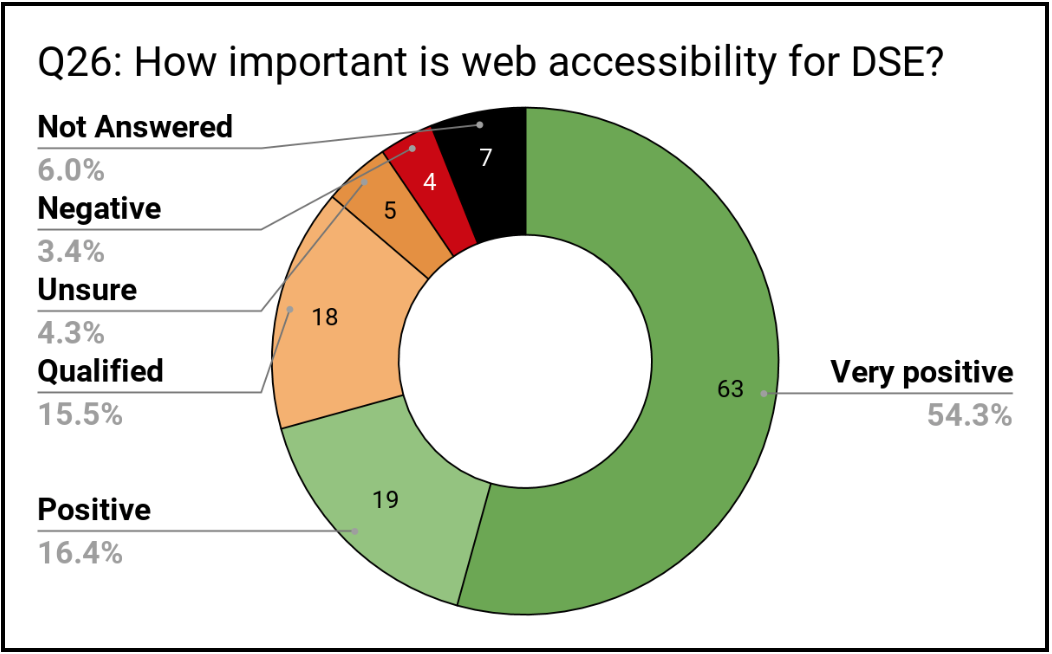
\includegraphics[width=\textwidth]{media/martinez5.png}
\caption{Distribution of importance assigned to web accessibility
in the design of DSE as analysed through Q26.}
\label{q26}
\end{figure}

Positive responses referred to the importance of catering to a broad
interpretation of the edition's target audience, an insufficient
awareness of the problem, a structural lack of resources and training,
the importance of considering accessible design at an early stage in the
project, and the fact that universal design improves user experience in
general --- not just that of people with disabilities. Most of the
critical responses referred to the difficulty and high cost of realizing
fully web accessible editions, and to the need for editors to prioritize
their efforts and expend their resources accordingly.\footnote{One
  critical respondent called web accessibility a ``luxury'' (R100).} In
some cases these arguments were justified by referring to the digital
scholarly editions' highly specialized target audience.

Most of the four negative responses we received were rather short, but
all indicated in some way or other that web accessibility is not (or
should not be) a priority in digital scholarly editing. One respondent
was more elaborate and expressed sentiments that recall some of the
statements made by the ``critical'' respondents, so it is quoted here in
full:
\begin{quote}
Not very. Ease of use and consideration of different access devices
(tablets, phones as well as traditional laptops, etc.) is part of the
design of all Web software. I don't think we need to supply specific
tools for say blind people to read our edition. First of all we're not
made of money and all this costs money. Someone who has an interest in
that sort of thing can do it instead.
\begin{flushright}
(R18)
\end{flushright}
\end{quote}
Again, the price of developing digital scholarly editions that are
accessible to people with disabilities is mentioned. The response
implies that editors should prioritize the development of their digital
scholarly editions to their target audience and suggests that people
with disabilities are not part of that target group. Instead, the burden
of developing digital scholarly editions that are web accessible (or
reengineering editions to make them more accessible) is pushed to an
external party. We should note that as a single response within a clear
minority of the survey's respondents, this is an outlier; however, the
opinion it expresses should be taken into consideration, especially
since it echoes several concerns voiced in the category of critical
responses. To conclude, we can say that while our survey suggests an
overwhelmingly positive attitude towards making digital scholarly
editions web accessible, the community also conversely indicates some
marked resistance towards its implementation. This implies that seven
years after Williams' essay, there is still a lack of awareness of these
issues among some members of the field.


\subsection{Diversity and inclusivity}

After exploring how digital scholarly editions can be made more
accessible to a wider group of people, we further extend the discussion
by examining what access can mean in terms of diversity and inclusivity.
As opportunities for the institutional support and development of
digital scholarship have proliferated, so too have calls for more
diverse and inclusive research groups and materials.\footnote{See for
  example Nell Smith 2007; \citealt{earhart_can_2012}; \citealt{fiormonte_towards_2012}; \citealt{liu_where_2012};
  \citealt{mcpherson_why_2012}; \citealt{risam_room_2013}; \citealt{risam_digital_2013}; \citealt{terras_changing_2013};
  \citealt{galina_russell_geographical_2014}; \citealt{bordalejo_diversity_2016}; Fiormonte 2016; \citealt{posner_whats_2016}; \citealt{eadh_diversity_2017}; \citealt{brown_ableism_2018}; \citealt{eichmann-kalwara_representation_2018}; \citealt{liu_digital_2018}; \citealt{losh_bodies_2018};
  \citealt{mahony_cultural_2018}; \citealt{risam_diversity_2018}, to name a few.}
Correspondingly, digital humanities scholars are continually confronted
with the difficulty of creating Internet-based research that is
simultaneously global and ethical, and are beginning to negotiate this
tension by engaging with scholars and materials not just from the Global
North, but also the Global South. However, this tension and its related
discourse seems to progress without notable input from the (mainly
European) digital scholarly editing community. This is remarkable,
because the symbiotic relationship between digital humanities and
digital scholarly editing, as well as editors' collaboration with
colleagues from disciplines that actively work toward social justice
(e.g. librarians and archivists), suggest that a critical reflection on
digital scholarly editing should address questions of inclusion and
diversity head-on.\footnote{On social justice as a core value of
  librarians, see \citealt[533-79]{rubin_foundations_2012}; \citealt{gustina_why_2017}. On
  social justice performed by archivists, see
  \citealt{jimerson_archives_2007}; \citealt{belmonte_archivists_2017}.} We therefore designed the inclusivity section of the
survey to gauge our respondents' familiarity with and opinions about
these issues and to add our community's voices to this discourse.

\begin{figure}[htb!]
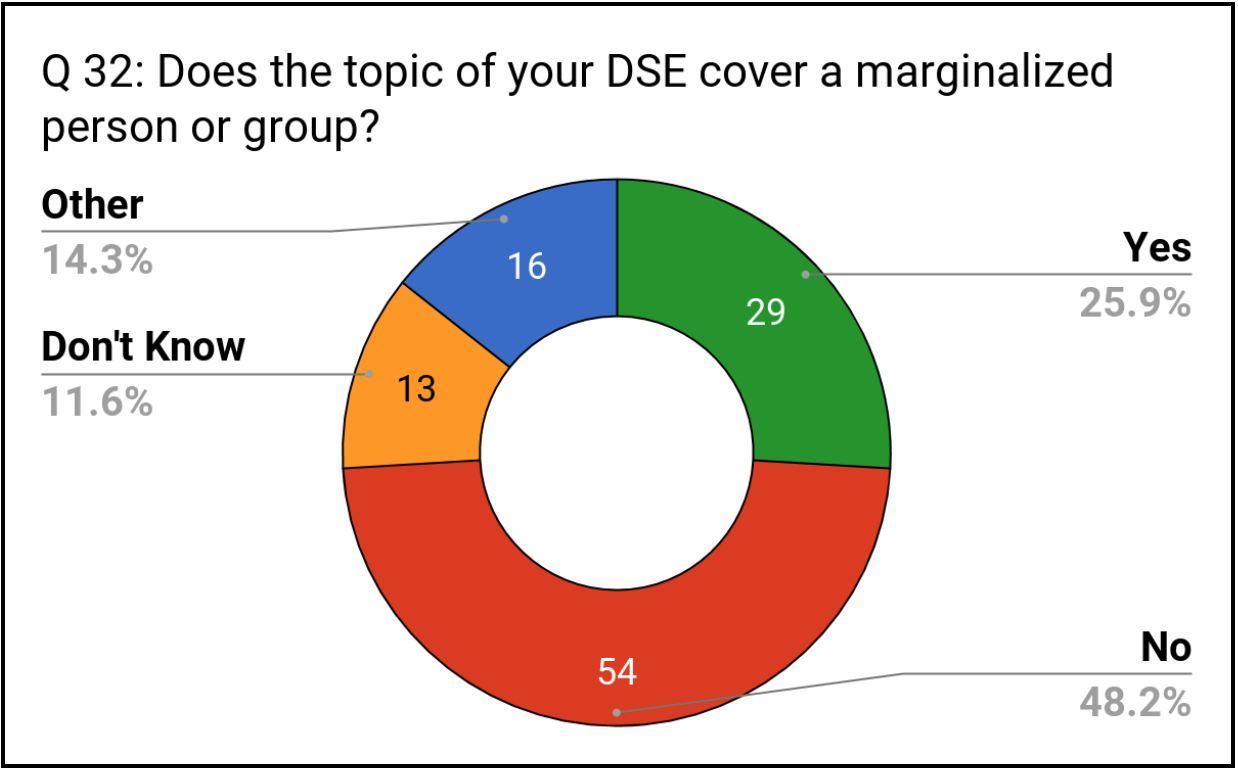
\includegraphics[width=\textwidth]{media/martinez6.png}
\caption{Response breakdown of Q32.}
\label{q32}
\end{figure}

As our own definition of inclusivity was focused on marginalized people
and groups, Q32 asked whether our respondents' editions covered such
material. A vast majority of our respondents (48.2\%, or 54 out of 112)
replied that theirs did not (see Figure \ref{q32}). Further context for this result was provided when respondents were asked whether or not inclusive
design (Q33) and subject matter (Q34) are prevailing concerns in the
development of digital scholarly editions. As the breakdown of these
questions in Figure \ref{q33} illustrates, in both cases the majority of
respondents answered that they are not prevailing concerns (49.1\% for
Q33; 42.2\% for Q34). Similarly, a minority of respondents argued that
it was not a concern, but that it should be (respectively seven and nine
respondents). We then asked respondents in Q35 and Q36 if they had any
opinions about what could be done to promote inclusive design and
inclusive subject matter, and received responses which generally
addressed three specific issues: collaboration, funding, and the
literary canon. Using responses from the survey, we explore these three
issues below.

\begin{figure}[p!]
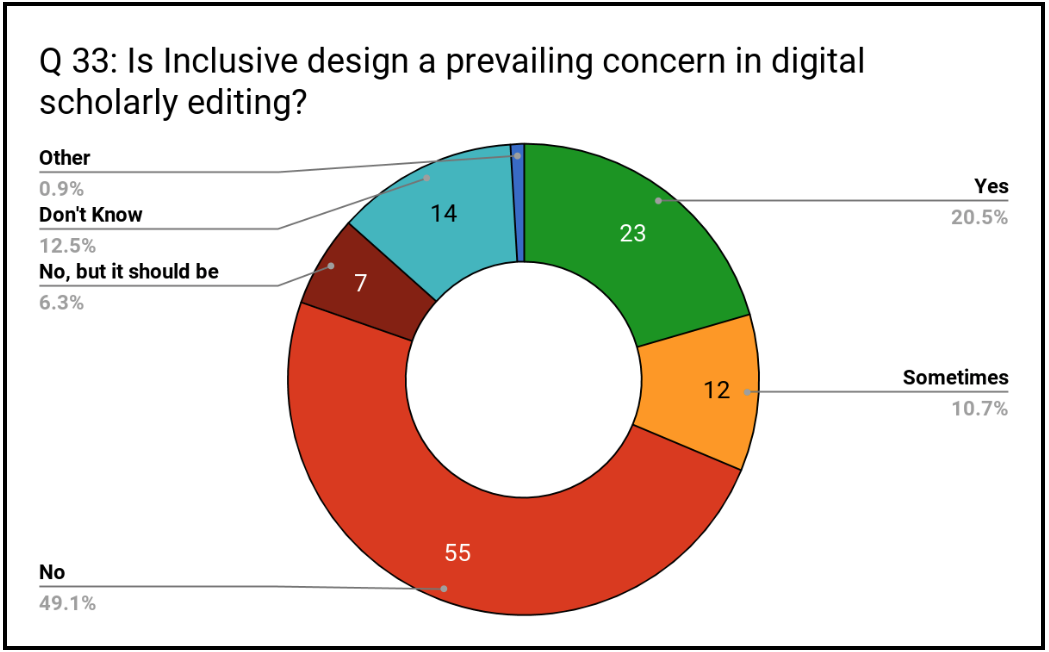
\includegraphics[width=\textwidth]{media/martinez7a.png}\\
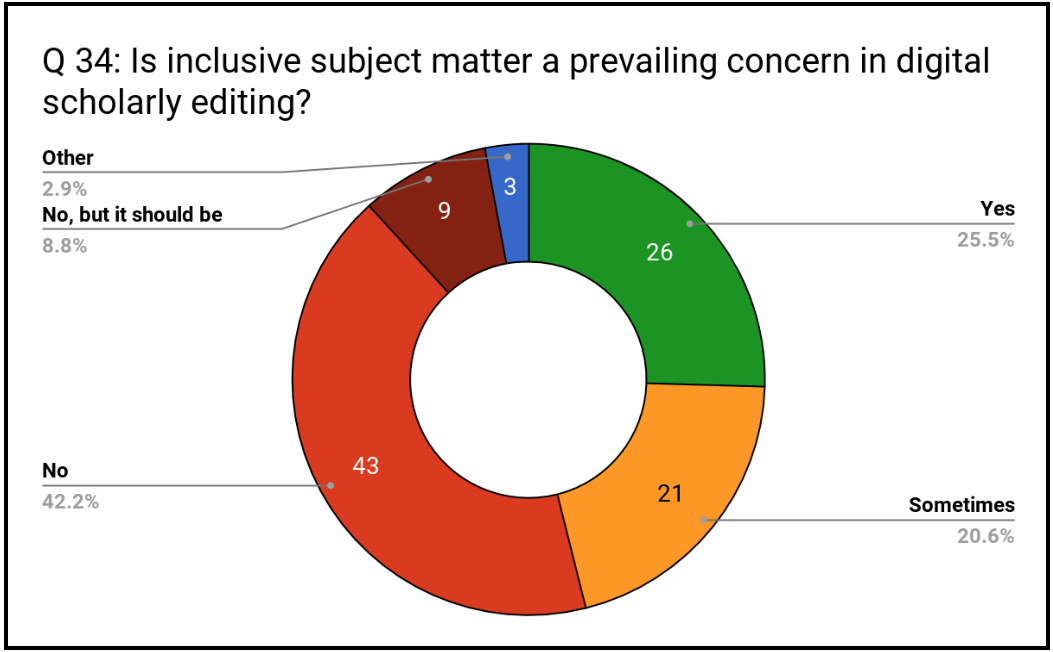
\includegraphics[width=\textwidth]{media/martinez7b.png}
\caption{Response breakdown of Q33 and Q34.}
\label{q33}
\end{figure}

In a recent paper Peter \citet[875]{robinson_project-based_2016} called for a
reconsideration of the role of editors to become ``key participants in,
and enablers of, communities'', rather than leaders of more exclusive
collaborations. Our respondents reinforced this claim, recommending that
in order to address issues of inclusion, more could be done to promote
and include diverse scholars and users, both in terms of traditionally
marginalized groups and in terms of diverse disciplinary backgrounds. As
R38 mentioned, digital scholarly editions need to ``have as diverse a
design, production, and dissemination team as possible. Diversity is
good in and of itself, especially if the team is demographically
simple''. R191 agreed, writing ``{[}a{]}s we gain diversity of the
people of the scholarly community the projects become more diverse,
too''. Another (R59) noted that ``marginalised people should be involved
in the process! Whether as editors or testing the DSEs before they go
live''. This sentiment was echoed by R14, who wrote that collaborative
editing projects should ``collect ideas/suggestions from a variety of
people (racial and ethnic groups, disabled and abled-bod{[}ied{]})''. It
is important to note, however, that the work of acknowledging and
confronting our implicit biases cannot be left solely to the user
community. While asking for user input is valuable and necessary, it
also shifts the burden of correcting issues of exclusion to those who
are being excluded, which can be exploitative. This needs planning
tempered with care and concern by editorial teams that choose to call
for user participation on these issues.

Over 50\% of our respondents commented that funding opportunities for
projects promoting diverse teams, exploring non-canonical authors and
materials, or for the inclusion of accessibility options in interface
design, are few and far between. As R131 observed, changing funding
policies is key to raising awareness around the issue of inclusion among
colleagues who may be resistant:

\begin{quote}
Raise awareness of the importance of the topic with funding and policy
setting bodies. I think researchers are plenty aware, but feel that
accessibility and inclusiveness is not a goal of research output. Also
aim awareness under 'techies'. The attitude of many technologists I know
is often quite rude and awareness is rudimentary. Like with the
misogynistic attitude inbred as sadly as it currently is in IT work,
also the topic of inclusiveness meets with knee jerk denial.
\end{quote}
R89 was one of many respondents who further reasoned that if funding
calls had requirements for inclusive design and subject matter, these
would become heightened areas of focus in digital scholarly editing:

\begin{quote}
I think it is a topic that is simply going to become unavoidable as time
goes on. I've been on grant panels where a failure to observe the
problem has led to grants being rejected out of hand by the committee.
That only has to happen a few times and people will pay more attention!
\end{quote}

Such responses underscore a key frustration in digital scholarship: the
expectation of researchers and users is that scholarly resources will be
available online, but, in comparison to the vast funding opportunities
for STEM, humanities researchers are given, as one respondent called it,
``peanuts'' (R131). There is then no doubt that actively designing
editions with questions of inclusivity and accessibility in mind can be
regarded as taking time away from content-building, particularly when
digital scholarly editors view themselves as creating digital resources
on a (relatively) shoestring budget within a tight time frame --- as was
corroborated in our section on web accessibility. The goal of digital
scholarly editing may then need a realignment of perspective, where
inclusive research is seen not as an afterthought or a box to be ticked,
but as a prime opportunity to explore new, untapped sources in
discipline-shaping ways.

Expanding funding for digital scholarly editing projects is linked to a
longer and equally critical process of expanding the (digital) literary
canon to include marginalized voices and themes. As R201 replied,

\begin{quote}
The funding bodies that support scholarly editions are still often
strongly motivated by theories of literary quality or cultural
significance in their funding decisions. While the wording of guidelines
may now provide fairly broad definitions of ``value'', nonetheless in
making funding decisions, canonical works are more likely to be
supported. These policies need explicit change.
\end{quote}
Literary quality is a subjective characteristic that can be ascribed to
texts by scholarly editors. As Hans Walter Gabler argues, ``editors can,
for sure, put works and texts, or indeed authors (of the past and
present), on the literary map, and within the ken of a general cultural
awareness'' and ``canonisation is intimately --- is, indeed,
functionally bound up with transmission'' \citeyearpar[366]{gabler_text_2018}. Actively seeking
out new texts and authors can contribute new understandings to our
editorial orientations --- or it can serve as the process by which we
discover new orientations \citep[see e.g.][]{van_hulle_orientations_2015}.
This in turn deepens and broadens our approach to the material we select
and explore, and potentially extends the possible applications of our
work. According to R190, broadening our scope of material could also be
a step toward ``acknowledging and addressing our dominant colonial and
imperialist culture''. It is important to clarify that marginalized
subject matter does not mean the same thing to every person in our
field. That is part of the tension around the topic. Respondents working
in medieval literature commented that they viewed the whole of their
subject as being marginalized, underused and under researched. A
respondent working in American literature replied, ``C19 American
Literature is all about marginalized voices'' (R129). Recognizing that
we have personal notions about what counts as ``marginalized'' is also a
recognition that there are multiple ways to approach this issue within
our respective time periods and subjects of study.
\section*{Moving forward}

In their introduction to \emph{Advances in Digital Scholarly Editing},
Peter Boot, Franz Fischer and Dirk Van Hulle argue that:

\begin{quote}
Scholarly editing has a long-standing tradition in the humanities. It is
of crucial importance within such disciplines as literary studies,
philology, history, philosophy, library and information science and
bibliography. Scholarly editors were among the first within the
humanities to realize the potential of digital media for performing
research, for disseminating their results, and for bringing research
communities together.

\begin{flushright}\citep[15-17]{boot_introduction_2017}\end{flushright}
\end{quote}

With such an illustrious history and a broad reach into other
disciplines, the field can be at the forefront of transforming the
digital edition into an environment that is as open, reproducible, and
inclusive as possible. Starting from a conviction that a reflexive,
collaborative and inclusive praxis is the cornerstone of good digital
scholarship, we designed this survey to determine to what extent
practitioners thought these issues were (or, indeed \emph{should be})
general concerns in the field.\footnote{As the survey's responses
  indicated, listening is a key factor in understanding where
  improvements can be made in academia: while conversations about how to
  refine aspects of praxis can be fraught with tension and disagreement,
  they are a necessary step in moving any discipline forward.} But what
the survey especially showed across all sections is that often
practitioners are not sufficiently aware of these issues to address them
in the first place.\footnote{Especially in the web accessibility and
  inclusivity sections many respondents either lamented a lack of
  awareness in the field or openly called for more awareness raising
  activities --- at times acknowledging that the survey itself had
  alerted them to new concerns that they hoped to take with them in the
  development of their editions.} Perhaps even more telling is that the
survey confirmed our hypothesis that the field is still grappling with
competing conceptions of access and accessibility.

When asked to define the concept of access with regard to the
dissemination and design of digital content (Q7), a majority of
respondents (127 out of 158, or just over 80\%) largely uniformly
defined it in terms of ``Open Access'' --- i.e. as content freely
accessible and openly available in a digital medium. Several respondents
emphasized the monetary aspect of this ``free'' availability, denouncing
the practice of putting up paywalls around scholarly content.\footnote{R129,
  for example, wrote: ``Not behind a paywall. Free as in beer'' --- a sly
  reference to Richard Stallman's well-known assertion that ```Free
  software' is a matter of liberty, not price. To understand the
  concept, you should think of `free' as in `free speech,' not as in
  `free beer''' \citeyearpar[3]{stallman_free_2002}.} Others stressed how important it is for
this content not only to be available, but also discoverable. Some
respondents also specifically mentioned inclusivity issues and the need
to cater to users with disabilities --- though we may have guided these
responses to some extent by highlighting these issues in the survey's
title and introduction. The issue becomes much more complex, however,
when we take a look at the definitions respondents wrote to describe the
concept of web accessibility (Q22). Although the term was defined at the
start of the survey, a considerable number of respondents were still
unfamiliar with it and understood the compound word literally --- as is
evident from responses such as: ``Accessible on the web? (R189), or
``{[}t{]}he way to be able to access DSE on the web?'' (R120).\footnote{The
  question marks at the end of these replies further indicate that the
  respondents were not confident in their definitions and were
  essentially uncertain about how to define the term.} And in many
cases, this concept was also defined in terms of discoverability or Open
Access.\footnote{R100 defined the concept as ``A big fight with
  copyright and estates''.} Nine respondents even indicated that they
made no distinction between the terms ``access'' and ``accessibility''
by explicitly referring to their definition in Q22.\footnote{See R19,
  R29, R35, R58, R59, R79, R104, R127 and R201.} A similar confusion of
terms occurs with the code of a digital scholarly edition: although
respondents were largely positive about the idea of accessible code, the
survey responses also showed considerable variation in the definition of
``code'', ranging from software to XML/TEI transcriptions. Accordingly,
there is little consensus in editorial strategies towards providing
sustainable access to the code of a digital scholarly edition. Finally,
it is striking that only just under half of the respondents (57 out of
123) explicitly refer to efforts that make editions more accessible to
people with disabilities. This again points to a great lack of awareness
in the field and implies that the term accessibility is used at cross
purposes. These are important factors to take into account when we try
to grasp the field's perspective on these issues.

As was suggested by the survey's respondents in its inclusivity section,
a key approach to raising awareness is through teaching. An extensive
and deep knowledge of editorial theory and practice is acquired with
time and experience, but how can we attract new talent? Introductions to
scholarly editing for a new generation of students often occurs in
summer schools and workshops. Such spaces can make inroads into
addressing ``marginalization'', by providing students with example
editions that meet the agreed definition of inclusion for that context
(though the cost of these schools in time and money can itself
marginalize interested parties). Often students develop further interest
in a field when they have a personal connection to the material and are
encouraged to question and analyze it from their own perspectives. This
can be accomplished by providing students with materials \emph{in which
they can see themselves}. We don't need to make assumptions about a
potential student's background, but the mere act of our choosing more
diverse texts by women, people of color, people with (in)visible
disabilities, people from the LGBTQIA+ community, and people who have
been marginalized for other political, religious and social reasons, is
a way of implicitly signifying that digital scholarly editing is a
discipline whose practitioners normalize such work and agree that it is
worthy of editorial attention. Making critical choices to include
teaching materials that showcase diverse content and inclusive design
can also provide new students with a baseline to develop skills in
cultural, web and software criticism, and to take up further calls to
expand the canon based on what sparks their own interests in ways that
are both interesting \emph{and} inclusive.

Given the conflicting understandings of terminology and the general need
for greater awareness of access issues, how do we move forward? We would
like this article to stand as a call to action, for the community to
come together to generate, and more importantly to implement, a set of
guidelines that address access in all its messy multiplicity, from
dissemination, to Open Access, code, web accessibility, and finally to
diversity. Such a call is neither unexpected nor unprecedented:
respondents mentioned several times that best practices are needed in
order to delineate clearly what is and should be expected of editors
with regard to access. There are well-considered guidelines for other
areas of our research, such as the TEI guidelines for XML, and the
\emph{RIDE} and MLA criteria for reviewing editions. These give us a
reference to return to when we want to evaluate our work against a
community standard. But establishing community standards for project
building around access, perhaps particularly where web accessibility and
inclusivity are concerned, will take careful, measured consideration, as
the survey responses indicate that these are murky waters. After
conducting this survey, it is clear that more specific research needs to
be done to investigate whether or not there is a demonstrable difference
in attitudes toward the digital (a ``digital divide'', so to speak)
between editors who have made the considerable theoretical and practical
move from the print paradigm and those who have only ever worked in the
digital. This could help explain the complexity of the approach to
concepts of access and accessibility in the editing community. Indeed,
much more could be done with our own dataset generated by this survey.
We don't profess to be statisticians and we recognize that others may
see connections where we did not. Therefore, we gladly offer a GDPR
compliant version of our questions and responses on Humanities Commons
for further review, reuse or remixing.

As fellows in a well-funded network on digital scholarly editing, we (as
authors) have enjoyed a great amount of privilege to explore the theory
and praxis of digital scholarly editing in the past four years. However,
such privilege needs to be considered when we (as a community) attempt
to design desiderata. What is actually feasible to achieve? This is up
to each editing team to decide for itself. We will never have uniformity
with regard to budgets, team size, project goals, computing power or
editorial approaches in our community. Such diversity is intellectually
stimulating. But having a set of guidelines and best practices
specifically about access and accessibility, which are generated by and
consider the needs of the marginalized as well as the privileged, the
precariously employed as well as the tenured, the ``digital migrants''
as well as the
``digital natives'', may provide an advantageous starting point for any
project, and, in turn, may help us become as diligent about the design
and dissemination of our digital scholarly editions as we are about the
transcription of our source materials.


\bibliography{references/martinez} 
\renewcommand{\thesubsection}{\thesection.\arabic{subsection}}  
\end{paper}
   
\contributor{
% Add all authors
Firstname Lastname, Firstname Lastname, etc.
}
\contribution{
% Add full title
Title. Subtitle.
}
\shortcontributor{
% short version of authors for running header
Lastname et al.
}
\shortcontribution{
% short version of title for running header
Title
}

\begin{paper}
\renewcommand*{\pagemark}{}

\begin{abstract}
\lipsum[1]
\end{abstract}
%\begin{motto}
% add a motto if you need one
%\end{motto}

% YOUR PAPER STARTS HERE

% remove asterisk (*) if you want to number your sections
\section*{Introduction} 
\lipsum[2]
\lipsum[3]

% remove asterisk (*) if you want to number your sections
\section*{Headings: first level}
% use \labels for inter-document references
\label{sec:Headings} 
\lipsum[4]

% remove asterisk (*) if you want to number your sections
\subsection*{Headings: second level}
By adding the previous label, you can now refer back to Section \ref{sec:Headings} and even dynamically say that this section starts on page \pageref{sec:Headings}.

% remove asterisk (*) if you want to number your sections
\subsubsection*{Headings: third level}
For your information, here is how you add footnotes.\footnote{Sample of the first footnote.}

\paragraph{Paragraph}
\lipsum[7]

% remove asterisk (*) if you want to number your sections
\section*{Examples figures and tables}
\label{sec:Others}
\lipsum[8] 

You can use ``in-text \textbf{citations}''\citep[see][5]{wiki:xx2}; see also \cite{wiki:xx2}. Or you can use block quotes:

\begin{quote}
LaTeX [...] is a document markup language and document preparation system for the TeX typesetting program. Within the typesetting system, its name is styled as \LaTeX. The term LaTeX refers only to the language in which documents are written, not to the editor used to write those documents. In order to create a document in LaTeX, a .tex file must be created using some form of text editor. While most text editors can be used to create a LaTeX document, a number of editors have been created specifically for working with LaTeX.

\citep{wiki:xx2}
\end{quote}

\subsection*{Figures}
See Figure \ref{fig:demographic}: 


\begin{figure}[H]
  \centering
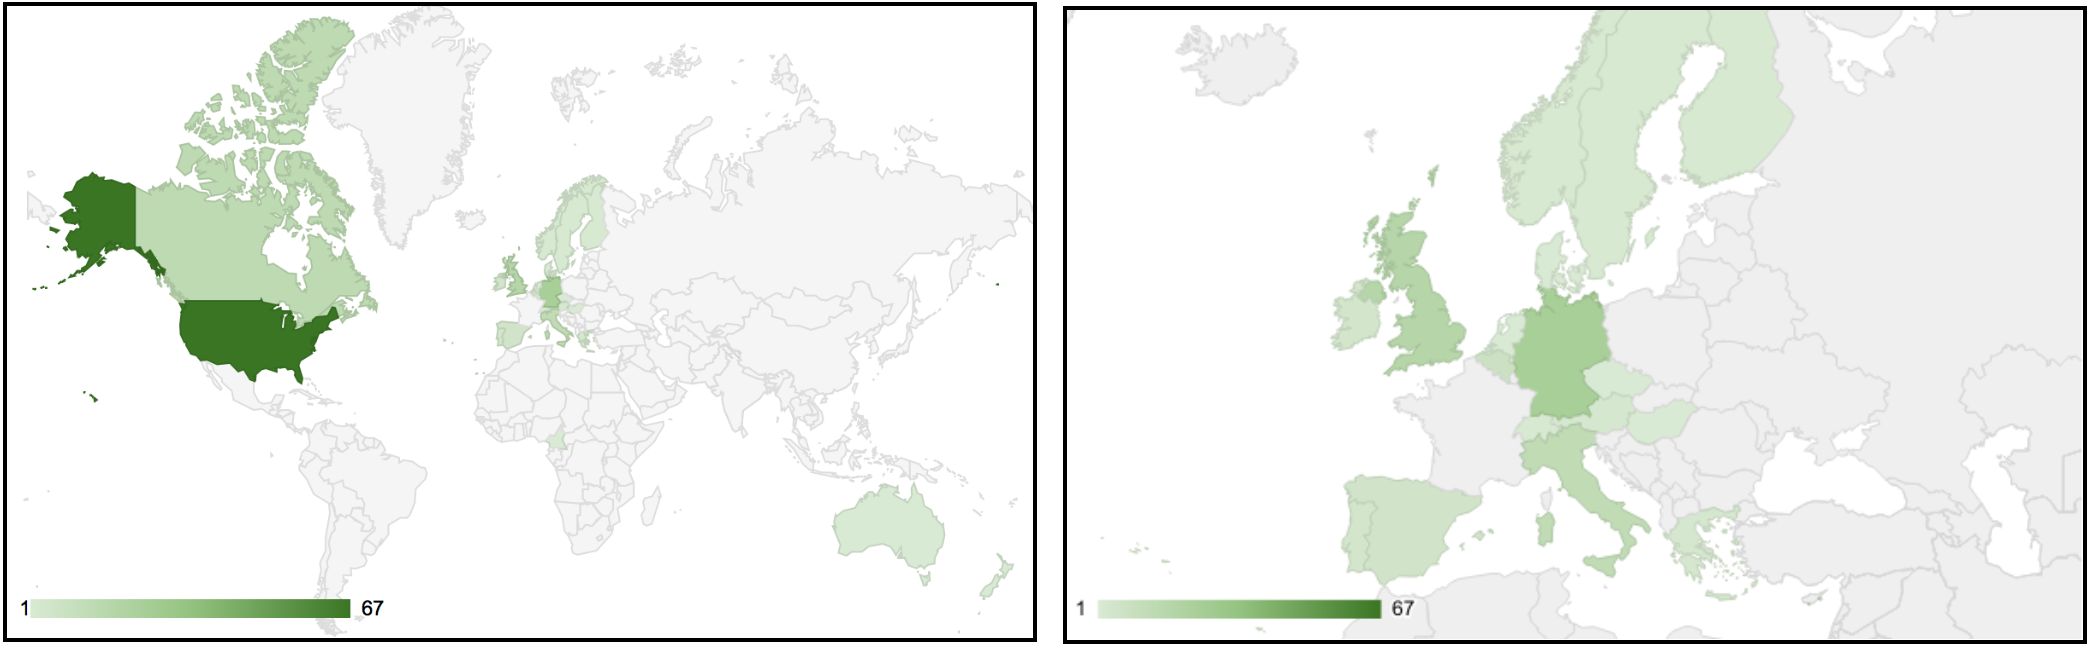
\includegraphics[width=\textwidth]{media/martinez1.png}  \caption{Sample figure caption.}
  \label{fig:demographic}
\end{figure}

\subsection*{Tables}
\lipsum[12]
See  Table~\ref{tab:table}.

\begin{table}[H]
 \caption{Sample table title}
  \centering
  \begin{tabular}{lll}
    \toprule
    \multicolumn{2}{c}{Part}                   \\
    \cmidrule(r){1-2}
    Name     & Description     & Size ($\mu$m) \\
    \midrule
    Dendrite & Input terminal  & $\sim$100     \\
    Axon     & Output terminal & $\sim$10      \\
    Soma     & Cell body       & up to $10^6$  \\
    \bottomrule
  \end{tabular}
  \label{tab:Table}
\end{table}


\bibliography{references/empty-template}  


\end{paper}
\part{Reviews}
%%%%%%%%%%%%%%
%% METADATA %%
%%%%%%%%%%%%%%

\contributor{
% your name(s)
Firstname Lastname
}

\contribution{
% complete information on the reviewed work
Reviewed Author, \emph{Reviewed Title}
}

\begin{review}
\renewcommand*{\pagemark}{}

%%%%%%%%%%%%%%%%%%%%%%%%%%%%%%%%%%%%%%
%% DESCRIPTION OF THE REVIEWED BOOK %%
%%%%%%%%%%%%%%%%%%%%%%%%%%%%%%%%%%%%%%

\begin{reviewed}
Review of \thecontribution. {[}Place{]}: {[}Publisher{]}, {[}Year{]}. {[}pages{]} pp. ISBN {[}number{]}. {[}Price{]}.
\end{reviewed}

%%%%%%%%%%%%%%%%%%%%%%%%%%%%%
%% YOUR REVIEW STARTS HERE %%
%%%%%%%%%%%%%%%%%%%%%%%%%%%%%

% remove asterisk (*) if you want to number your sections
% add a title for your section in between the {curly brackets} if you need one
\section*{} 
Your Review \citep{key}.

\begin{flushleft}
    % use smallcaps for author names
    \renewcommand*{\mkbibnamefamily}[1]{\textsc{#1}}
    \renewcommand*{\mkbibnamegiven}[1]{\textsc{#1}} 
\printbibliography
\end{flushleft}

% safeguard section numbering
\renewcommand{\thesubsection}{\thesection.\arabic{subsection}} 
\end{review}
\contributor{Wout Dillen}
\contribution{My Pretty Lorem Ipsum Paper. A Paper for the Ages.}
\shortcontributor{Dillen}
\shortcontribution{My Pretty Lorem Ipsum Paper}

\begin{paper}
\renewcommand*{\pagemark}{}

% Start with the abstract
% FYI: delete \lipsum commands as you fill in the text
\begin{abstract}
\lipsum[1]
\end{abstract}
\begin{motto}
They say that every paper should have a motto. They are probably wrong.

(Dillen 2019)
\end{motto}

% YOUR PAPER STARTS HERE
% ALWAYS start with \section{}, to make sure the first paragraph is not indented
% Keep \section{} empty if you don't want a section title
% Add an asteriks to \section*{} if you don't want it to have a section number
% (the same goes for \subsection*{} and \subsubsection*{}

% In other words: if you just want to start writing without any titles, just put down:
% \section*{} 
% and start writing

% put the first 3-4 words inside \textsc{} for small caps

\section{Introduction}
\lipsum[2]
\lipsum[3]


\section{Headings: first level}
\label{sec:headings}

\lipsum[4] See Section \ref{sec:headings}.

\subsection{Headings: second level}
\lipsum[5]
\begin{equation}
\xi _{ij}(t)=P(x_{t}=i,x_{t+1}=j|y,v,w;\theta)= {\frac {\alpha _{i}(t)a^{w_t}_{ij}\beta _{j}(t+1)b^{v_{t+1}}_{j}(y_{t+1})}{\sum _{i=1}^{N} \sum _{j=1}^{N} \alpha _{i}(t)a^{w_t}_{ij}\beta _{j}(t+1)b^{v_{t+1}}_{j}(y_{t+1})}}
\end{equation}

\subsubsection{Headings: third level}
\lipsum[6]

\paragraph{Paragraph}
\lipsum[7]

\section*{Examples of citations, figures, tables, references}
\label{sec:others}
\lipsum[8] \citep{wiki:xxx} and see \cite{wiki:xxx}.

The documentation for \verb+natbib+ may be found at
\begin{center}
  \url{http://mirrors.ctan.org/macros/latex/contrib/natbib/natnotes.pdf}
\end{center}
Of note is the command \verb+\citet+, which produces citations
appropriate for use in inline text.  For example,
\begin{verbatim}
   \citet{hasselmo} investigated\dots
\end{verbatim}
produces
\begin{quote}
  Hasselmo, et al.\ (1995) investigated
\end{quote}

\begin{center}
  \url{https://www.ctan.org/pkg/booktabs}
\end{center}
Also useful is the \verb+lstlisting+ envrironment, which lets you produce code, like this \verb+bash+ example:
\begin{lstlisting}[language=bash]
#some comment about changing directories
cd Documents
\end{lstlisting}
Or even \verb+XML+:
\begin{lstlisting}[language=XML]
<parent name="TEI">
    <child>TEI Simple</child> <!--Pretty?-->
</parent>


\end{lstlisting}

\subsection*{Figures}
\lipsum[10] 
See Figure \ref{fig:fig1}. Here is how you add footnotes.\footnote{Sample of the first footnote.}
\lipsum[11] 

\begin{figure}[H]
  \centering
  \fbox{\rule[-.5cm]{4cm}{4cm} \rule[-.5cm]{4cm}{0cm}}
  \caption{Sample figure caption.}
  \label{fig:fig1}
\end{figure}

\subsection*{Tables}
\lipsum[12]
See awesome Table~\ref{tab:table}.

\begin{table}[H]
 \caption{Sample table title}
  \centering
  \begin{tabular}{lll}
    \toprule
    \multicolumn{2}{c}{Part}                   \\
    \cmidrule(r){1-2}
    Name     & Description     & Size ($\mu$m) \\
    \midrule
    Dendrite & Input terminal  & $\sim$100     \\
    Axon     & Output terminal & $\sim$10      \\
    Soma     & Cell body       & up to $10^6$  \\
    \bottomrule
  \end{tabular}
  \label{tab:table}
\end{table}

\subsection*{Lists}
\begin{itemize}
\item Lorem ipsum dolor sit amet
\item consectetur adipiscing elit. 
\item Aliquam dignissim blandit est, in dictum tortor gravida eget. In ac rutrum magna.
\end{itemize}
\bibliography{references/example-template}  

\end{paper}
\appendix
% add Author Agreement section as a \part in the ToC
\addcontentsline{toc}{part}{Author Agreement template}
% use "authors" style for headers and footers
\pagestyle{empty}
% format "Authors" section as a new \chapter
\section*{Author Agreement to Publish a Contribution as Open-Access on \thewebsite}


In this document, the “Editors” refers to:
\begin{enumerate}
    \item editor 1
    \item editor 2
    \item etc
\end{enumerate}

\vskip 1em

\noindent In this document, the “Author(s)” refers to:
\begin{enumerate}
    \item author 1
    \item author 2
    \item etc
\end{enumerate}

\vskip 1em

\noindent This is an Agreement between {[}name{]} (the “Corresponding Author”), and \thejournal \ (the “Journal”), concerning the publication of {[}title{]} (the “Contribution”) in \theissue \ (the “Volume”). 

The Author(s) agree(s) that the Contribution shall be made available as an open-access publication under the \doclicenseLongNameRef \ (\doclicenseNameRef) \ license, available at \doclicenseURL \ (the “License”), and be published as part of the Volume.

The Author(s) agree(s) that copies of the Contribution in \verb+.pdf+, and \verb+.html+ formats are made publicly available under the aforementioned License on the servers of the Journal and deposited in relevant public repositories. 

The Author(s) grant(s) the Editors of the Journal and the organizations archiving the Journal the non-exclusive and irrevocable right to archive their contribution and to make it accessible (online and free of charge) for public distribution. 

This granted right extends to any associated metadata of the Contribution. Specifically, the Author(s) license the associated metadata under a Creative Commons CC0 1.0 Universal license (public domain). The Author(s) agree that their author name(s) and affiliation(s) are part of the associated metadata and may be stored on the servers of the Journal and made available under the CC0 license. The Author(s) acknowledge that the Editors hold the copyright for the Volume. Please tick the relevant box: 

\begin{enumerate}
    \item ( \ ) The Contribution does not include any third-party material such as figures, code, data sets and others. 
    \item ( \ ) The Contribution does include third-party material such as figures, code, data sets and others. The Author(s) warrant that they have the right to include these materials in the Contribution. The Author(s) attach a copy/scan of applicable agreement(s) of the rights holders to this Agreement. The Author(s) warrant that the Contribution (including any accompanying material such as data sets) does not infringe any rights of third parties, for example trademark rights, privacy rights, and intellectual property rights. 
\end{enumerate}

The Author(s) understand that they retain the copyright to the Contribution. They understand that the dedication of the Contribution under the License is irrevocable. They understand and agree that the full responsibility/liability for the content of the contribution rests upon them as the Author(s) of the Contribution. The Author(s) release the Editors, persons providing the \thejournal \ service, and the organizations archiving the Journal from any liability caused by the publication or archiving of the Contribution via the servers used for the Journal. 

The Author(s) have read the conditions of the License and agree to apply it to the Contribution. 

The Corresponding Author hereby confirms that all of the Authors have read this Agreement, and agree to its terms.

The Corresponding Editor hereby confirms that all of the Editors have read this Agreement, and agree to its terms.

\vskip 2em

\noindent The Corresponding Editor:\\
Location:\\
Date:\\
Signature:\\

\vskip 4em

\noindent The Corresponding Author:\\
Location:\\
Date:\\
Signature:\\


% add Authors section as a \part in the ToC
\addcontentsline{toc}{part}{Authors}
% use "authors" style for headers and footers
\pagestyle{authors}
% format "Authors" section as a new \chapter
\chapter*{Authors}
% pagenr at the bottom
\protect\thispagestyle{plain.authors}

% Short Bios of authors start here
% Each author gets 1 \paragraph
% Each \paragraph starts with author name
% This author name is formatted as the \paragraph title to make it pop out more (bold and some space)


\paragraph{Elli Bleeker} is a postdoctoral researcher in the Research and Development Team at the Humanities Cluster, part of the Royal Netherlands Academy of Arts and Sciences. She specializes in digital scholarly editing and computational philology, with a focus on modern manuscripts and genetic criticism. Elli completed her PhD in 2017 at the University of Antwerp on the role of the scholarly editor in the digital environment. During her Early Stage Research Fellowship in the Marie Skłodowska-Curie funded DiXiT network (2014–2017), she received advanced training in manuscript studies, text modeling, and XML technologies. She has participated in the organization and teaching of workshops on scholarly editing with a focus on knowledge transfer and the application of computational methods in a humanities environment. She is also the Associate Editor of Variants from this issue onwards.

\paragraph{Wout Dillen} holds a PhD in Literature with a focus on text encoding and digital scholarly editing from the University of Antwerp. From 2016 to 2017, Wout held a Marie Skłodowska-Curie Experienced Research Fellowship in the Digital Scholarly Editions Initial Training Network (DiXiT ITN) at the University of Borås. Since 2016 he has been the Coordinator of platform{DH} and the Coordinator of the University of Antwerp’s contribution to DARIAH-Flanders. Wout currently serves as the Secretary of the European Society of Textual Scholarship (ESTS), as a member of the Steering Committee of the DH Benelux. For the current issue, Wout is an Associate editor of Variants, and will be General Editor from issue 15 onwards. Besides these, he is also on the editorial boards of the Review Journal for Digital Editions and Resources (RIDE) and the upcoming DH Benelux journal.

\paragraph{Aodhán Kelly} is an affiliated researcher in the Centre for Manuscript Genetics at the University of Antwerp and was a Marie Skłodowska-Curie Early Stage Research Fellow within the DiXiT network. Aodhán researches methods and models for the dissemination of digital scholarly editions to wider audiences and he defended a PhD thesis on this topic at the University of Antwerp in July 2017 with the title ``Disseminating digital scholarly editions of textual cultural heritage''.

\paragraph{Merisa Martinez} is a PhD Candidate in the Swedish School of Library and Information Science at the University of Borås, a Visiting Research Fellow at the Cambridge Digital Library, and a member of the Program Committee for the 2019 Digital Access to Textual Cultural Heritage (DaTech) Conference. From 2014 to 2017, she held a Marie Skłodowska-Curie Early Stage Research Fellowship in the Digital Scholarly Editions Initial Training Network (DiXiT ITN), where she also served for three years as an elected Student Representative to the Project Advisory Board. Merisa is currently writing a doctoral dissertation on the intersection of digital textual scholarship and the digitization process in libraries, which she will defend in 2019.

\paragraph{Anna-Maria Sichani} is a Research Fellow in Media History and Historical Data Modelling on the AHRC-funded ‘Connected Histories of the BBC’ project at the Department of Media, Film and Music at University of Sussex and Sussex Humanities Lab. In 2018, she completed her PhD in Modern Greek Philology and Cultural Studies at University of Ioannina in Greece. From 2017 to 2018, Anna-Maria was the Communications Fellow for the Alliance of Digital Humanities Organizations (ADHO). Previously, Anna-Maria held a Marie Skłodowska-Curie Early Stage Research Fellowship in the Digital Scholarly Editions Initial Training Network (DiXiT ITN) at Huygens ING and a PhD Research Fellowship at King’s College Digital Lab in London. She has collaborated on a number of Digital Humanities projects including the COST Action “Distant Reading for European Literary History," Transcribe Bentham, and DARIAH. Currently, Anna-Maria serves on the Editorial Board of The Review Journal for Digital Editions and Resources (RIDE) and at The Programming Historian.
\end{document}